\documentclass[twocolumn,5p,sort&compress]{elsarticle}
\pdfoutput=1
\usepackage{url}
\usepackage{tikz}
\usepackage{comment}
\usepackage{framed,graphicx}
\usepackage{multirow}
\usepackage{rotating}
\usepackage{amsmath}
\usepackage{bigstrut}
\usepackage{color}
\usepackage{graphics}
\usepackage{eqparbox}
\usepackage{graphics}
\usepackage{colortbl}
\usepackage{paralist}
\usepackage{soul}
\usepackage{xcolor}
\usepackage{caption}
%\usepackage{times}
\usepackage{mathptmx} 
\usepackage{courier}
\usepackage{balance}
\usepackage{picture}
\usepackage{algorithm}
\usepackage{algorithmicx}
\usepackage{algpseudocode}
\usepackage[export]{adjustbox}
\definecolor{lightgray}{gray}{0.8}
\definecolor{darkgray}{gray}{0.6}
\definecolor{lavenderpink}{rgb}{0.98, 0.68, 0.82}
\definecolor{celadon}{rgb}{0.67, 0.88, 0.69}
\renewcommand{\algorithmicrequire}{\textbf{Input:}}
\renewcommand{\algorithmicensure}{\textbf{Output:}}
%%% graph
\newcommand{\crule}[3][darkgray]{\textcolor{#1}{\rule{#2}{#3}}}

\newcommand{\quart}[4]{\begin{picture}(80,4)%1
	{\color{black}\put(#3,2){\circle*{4}}\put(#1,2){\line(1,0){#2}}}\end{picture}}

\definecolor{Gray}{gray}{0.95}
\definecolor{LightGray}{gray}{0.975}

%% timm tricks
\newcommand{\tion}[1]{{\S}\ref{sect:#1}}
\newcommand{\eq}[1]{Equation~\ref{eq:#1}}
\newcommand{\fig}[1]{Figure~\ref{fig:#1}}
\newcommand{\bi}{\begin{itemize}}
\newcommand{\ei}{\end{itemize}}
\newcommand{\be}{\begin{enumerate}}
\newcommand{\ee}{\end{enumerate}}
\usepackage{enumitem}
\setitemize{noitemsep,topsep=0pt,parsep=0pt,partopsep=0pt}

  \biboptions{sort&compress}

\definecolor{steel}{rgb}{.11, .11, .7}
\definecolor{Gray}{rgb}{0.88,1,1}
\definecolor{Gray}{gray}{0.85}
\usepackage[framed]{ntheorem}
\usetikzlibrary{shadows}
\theoremclass{Lesson}
\theoremstyle{break}

% inner sep=10pt,
\tikzstyle{thmbox} = [rectangle, rounded corners, draw=black,
fill=Gray!40,  drop shadow={fill=black, opacity=1}]
\newcommand\thmbox[1]{%
	\noindent\begin{tikzpicture}%
	\node [thmbox] (box){%
		\begin{minipage}{.94\textwidth}%
		\vspace{-2mm}#1\vspace{-3mm}%
		\end{minipage}%
	};%
	\end{tikzpicture}}

\let\theoremframecommand\thmbox
\newshadedtheorem{lesson}{Result}



\begin{document}
\begin{frontmatter}

\title{What is  Wrong with
Topic Modeling? (and How to Fix it Using Search-based Software Engineering)}



\author{Amritanshu Agrawal\corref{cor1}}

\cortext[cor1]{Corresponding author: Tel: +1-919-637-0412 (Amritanshu)}

\ead{aagrawa8@ncsu.edu}
\ead[url]{http://ai4se.net/}

\author{Wei Fu\corref{cor1}}
\ead{wfu@ncsu.edu}

\author{Tim Menzies\corref{cor1}}
\ead{tim.menzies@gmail.com}
\address{Department of Computer Science, North Carolina State University, Raleigh, NC, USA}

\begin{abstract}

\noindent \textbf{Context:} Topic modeling finds
  human-readable structures in unstructured textual data. A
  widely used topic modeler is Latent Dirichlet allocation. When
  run on different datasets, LDA suffers from ``order effects''
  i.e.
 different topics are generated if the order of training data is shuffled.
  Such order effects introduce a
 systematic error for any study. This error can relate to misleading results;
  specifically, inaccurate topic descriptions and a reduction in the efficacy of
  text mining classification results.

 \noindent
\textbf{Objective:} To provide a method in which distributions
generated by LDA are more stable and can be used for further analysis.

 \noindent
\textbf{Method:} We use LDADE, a search-based software engineering tool that tunes LDA's parameters using DE 
(Differential Evolution).
LDADE is evaluated on data from a programmer
information exchange site (Stackoverflow), title and abstract text of thousands
of Software Engineering (SE) papers, and software defect reports from NASA. Results were collected
across different implementations of LDA (Python+Scikit-Learn, Scala+Spark); across
different platforms (Linux, Macintosh) and for different kinds of LDAs (VEM, or using Gibbs sampling). 
Results were scored via topic stability and text mining classification accuracy.

\noindent
\textbf{Results:}
In all treatments:
   (i)~standard LDA exhibits very large topic instability;
  (ii)~LDADE's tunings dramatically reduce cluster instability; 
  (iii)~LDADE also leads to  improved performances for supervised as well as unsupervised learning.

\noindent
\textbf{Conclusion:}
  Due to topic instability,
  using standard LDA with its ``off-the-shelf'' settings should now be depreciated.
  Also, in future,
we should require
SE
papers that use
LDA
to
test and (if needed) mitigate LDA topic instability.
  Finally, LDADE is a candidate technology for effectively and efficiently reducing that instability.  
\end{abstract}

\begin{keyword}
Topic modeling, Stability, LDA, tuning, differential evolution.
\end{keyword}

\end{frontmatter}



\section{Introduction}
\label{sect:intro} 

The current great challenge in software analytics
is understanding unstructured data. As shown in Figure~\ref{fig:
data}, most of the planet's 1600 Exabytes of data does not appear
in structured sources (databases, etc)~\cite{nadkarni2014structured}.
Rather it is {\em unstructured} data, often in free text, and found
in word processing files, slide presentations, comments, etc.

Such unstructured data does not have a pre-defined data model and
is typically text-heavy. Finding insights among unstructured text
is  difficult unless we can search, characterize, and classify the
textual data in a meaningful way. One of the common techniques for
finding related topics within unstructured text (an area called
topic modeling) is Latent Dirichlet allocation (LDA)~\cite{blei2003latent}.

This paper explores systematic errors in LDA analysis.
LDA is a non-deterministic algorithm since its internal weights are updated via a stochastic sampling process (described
later in this paper).
We show in this paper that this non-determinism means that the  topics generated by LDA on
SE data are subject to order effects; i.e. different input orderings
can lead to different topics.
Such instability can:
\bi
\item
  Confuse users when they see different topics each time
the algorithm is re-run) 
\item
  Reduce the efficacy of text mining classifiers that rely on LDA to
  generate their input training data.
\ei
To fix this problem,
we propose LDADE: a  combination of LDA and a search-based optimizer (differential evolution, or DE)~\cite{storn1997differential})
that automatically tunes LDA's \mbox{$<k$, $\alpha$, $\beta>$} parameters. This paper tests LDADE 
by applying text mining to
three data sets:
\be
\item Data from a programmer information exchange site (Stackoverflow);
  \item Title and abstract text of
    15121 SE papers;
  \item Software defect reports from NASA.
\ee
    
\noindent
Using these datasets, we explore these research questions:  
   
\bi

\item \textbf{RQ1}: \textbf{Are the default settings of LDA incorrect?} We will show that using the default settings of LDA for SE data can lead to systematic errors since stability scores start to drop after $n=5$ terms per topic.
    \item \textbf{RQ2}: \textbf{Does LDADE improve the stability scores?} LDADE dramatically improves stability scores using
      the parameters found automatically by DE. 
    \item \textbf{RQ3}: \textbf{Does LDADE improve text mining classification accuracy?} 
      Our experiments shows that LDADE  also improves classification accuracy.
    \item \textbf{RQ4}: \textbf{Do different data sets
      need different configurations to make LDA stable?} LDADE finds different ``best'' parameter settings for different data sets. Hence reusing tunings  suggested  by  any other  previous study  for any dataset is \underline{{\em not}} recommended. Instead,  it is better to
      use  automatic  tuning  methods  to find the best tuning parameters for the current data set.
      \item \textbf{RQ5}: \textbf{Are our findings consistent using different kinds of LDA or with different implementations?} Results were collected across different implementations of LDA and across different platforms (Linux, Macintosh) and for different kinds of LDAs. Across all these implementations,
        the same effect holds: (a)~standard LDA suffers from order effect and topic instability
        and (b)~LDADE can reduce that instability.
    \item \textbf{RQ6}: \textbf{Is tuning easy?} We show that, measured
      in the terms of the internal search space of the optimizer,
      tuning LDA is much simpler than standard optimization methods.
    \item \textbf{RQ7}: \textbf{Is tuning extremely slow?}
      The advantages of  LDADE come at some cost:
      tuning with DE makes LDA three to five times slower.
      While this is definitely more than not using LDA, this may not be an arduous increase
      given modern cloud computing environments. 
    \item \textbf{RQ8}: \textbf{Should topic modeling be used ``off-the-shelf'' with their default tunings?}
      Based on these findings, our answer to this question is an emphatic ``no''. We can see little reason to use ``off-the-shelf'' LDA for any kind of SE data mining applications.
      \ei
\begin{figure}[!t]
  \captionsetup{justification=centering}
  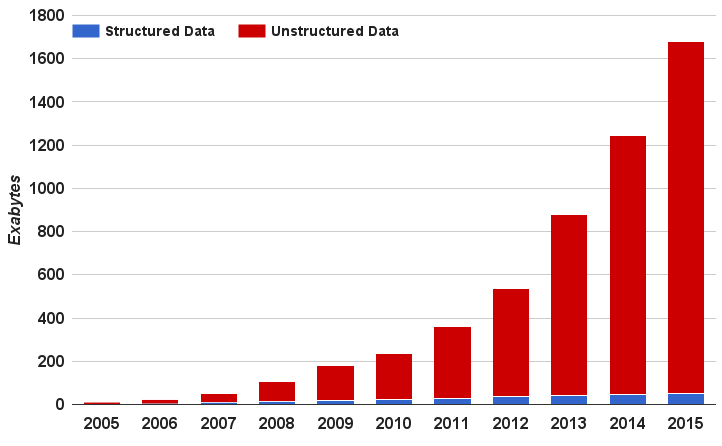
\includegraphics[width=\linewidth]{./fig/data.png}
  \caption{Data Growth 2005-2015. From~\cite{nadkarni2014structured}.}
  \label{fig: data}
\end{figure}
The rest of this paper is structured as follows.
\tion{motivate} argues that stabilizing the topics generated by LDA is important for several reasons.
%\be
%\item
%LDA is widely used so it is important to study how to use it better;
%\item
%A  lack of stability  in LDA topics raises doubts about some prior
%research results;
%\item
% Improving LDA topic stability improves classification accuracy; 
% \ee
Related work is revised in \tion{related} and the methods of this paper are discussed in \tion{evaluation}.
We have answered above research questions in
\tion{results}. This is followed by a discussion on the validity of our results and a section
describing our conclusions.
Note that the main conclusion
of this paper is that, henceforth,
we should require
SE
papers that use
LDA
to
test and (if needed) mitigate LDA topic instability.
\section{Motivation}
\label{sect:motivate}

\begin{table}[!b]
\renewcommand\arraystretch{1.0}
\begin{center}
\scriptsize
\begin{tabular}{|c|l|c|}
\hline
\begin{tabular}[c]{@{}c@{}}\textbf{Venue}\end{tabular} & \begin{tabular}[c]{@{}c@{}}\textbf{Full Name}\end{tabular}     & \multicolumn{1}{l|}{\textbf{Count}} \\ \hline
ICSE & International Conference on Software Engineering  & 4  \\ \hline
\begin{tabular}[c]{@{}c@{}}CSMR-\\WCRE\\ / SANER \end{tabular}   & \begin{tabular}[c]{@{}l@{}}International Conference on Software Maintenance,\\ Reengineering, and Reverse Engineering / International \\Conference on Software Analysis,Evolution, and \\Reengineering\end{tabular} & 3  \\ \hline
\begin{tabular}[c]{@{}c@{}}ICSM\\ / ICSME\end{tabular}   & \begin{tabular}[c]{@{}l@{}}International Conference on Software Maintenance / \\International Conference on Software Maintenance and \\Evolution \end{tabular}  & 3\\ \hline
ICPC & International Conference on Program Comprehension  & 4  \\ \hline
ASE      & \begin{tabular}[c]{@{}l@{}}International Conference on Automated Software\\ Engineering  \end{tabular} & 3  \\ \hline
ISSRE      & \begin{tabular}[c]{@{}l@{}}International Symposium on Software Reliability\\ Engineering \end{tabular} & 2  \\ \hline
MSR      & \begin{tabular}[c]{@{}l@{}}International Working Conference on Mining \\Software Repositories \end{tabular} & 8  \\ \hline
OOPSLA  & \begin{tabular}[c]{@{}l@{}}International Conference on Object-Oriented \\Programming, Systems, Languages, and Applications \end{tabular}  & 1 \\ \hline
FSE/ESEC  &  \begin{tabular}[c]{@{}l@{}}International Symposium on the Foundations of Software \\Engineering / European Software Engineering Conference \end{tabular}  & 1                                    \\ \hline
TSE                                 & IEEE Transaction on Software Engineering   & 1                                     \\ \hline
IST                                 & Information and Software Technology                                 & 3                                       \\ \hline
SCP                                 & Science of Computer Programming                               & 2                                       \\ \hline
ESE                                 & Empirical Software Engineering                         & 4                                       \\ \hline
\end{tabular}
\end{center}
\caption{SE Venues that publish  on Topic Modeling.}
\label{tab:venues}
\end{table}

   
\renewcommand\arraystretch{1.2}
\begin{table*}[!t]
\scriptsize
\centering
    \begin{tabular}{|c@{~}|c@{~}|c@{~}|c@{~}|c@{~}|c@{~}|c@{~}|p{5.7cm}@{~}|p{3.5cm}|}
        \hline 
        \begin{tabular}[c]{@{}c@{}}\textbf{ID}\end{tabular} & \textbf{Year} & \textbf{Citations} & \textbf{Venues} & \begin{tabular}[c]{@{}c@{}}\textbf{Mentions} \\\textbf{instability} \\\textbf{in LDA?} \end{tabular} &\begin{tabular}[c]{@{}c@{}} \textbf{Uses} \\\textbf{Default} \\\textbf{Parameters}\end{tabular}&\begin{tabular}[c]{@{}c@{}} \textbf{Does} \\\textbf{tuning?}\end{tabular} & \multicolumn{1}{c|}{Conclusion}  & \multicolumn{1}{c|}{Tasks / Use cases}\\ \hline
        \cite{rao2011retrieval} & 2011 & 112 & WCRE & Y & Y & N & \begin{tabular}[c]{@{}l@{}}Explored Configurations without any explanation. \end{tabular} & \begin{tabular}[c]{@{}l@{}}Bug Localisation\end{tabular}\\ [0.5ex]\hline
        \cite{oliveto2010equivalence} & 2010 & 108 &MSR& Y & Y & N & \begin{tabular}[c]{@{}l@{}}Explored Configurations without any explanation.\\ Reported their results using multiple experiments.\end{tabular}& \begin{tabular}[c]{@{}l@{}}Traceability Link recovery\end{tabular}\\ [0.5ex]\hline
        \cite{barua2014developers} &2014& 96 & ESE & Y & Y & N  & \begin{tabular}[c]{@{}l@{}}Explored Configurations without any explanation.\\ Choosing right set of parameters is a difficult task.\end{tabular}& \begin{tabular}[c]{@{}l@{}}Stackoverflow Q\&A data analysis\end{tabular}\\ [0.5ex]
        \hline
        \cite{panichella2013effectively} & 2013&75&ICSE & Y & Y & Y  & \begin{tabular}[c]{@{}l@{}}Uses GA to tune parameters. They determine\\ the near-optimal configuration for LDA in the \\context of only some important SE tasks.\end{tabular}& \begin{tabular}[c]{@{}l@{}}Finding near-optimal configurations\end{tabular}\\ [0.5ex]
        \hline
        \cite{galvis2013analysis} &2013& 61 &ICSE& Y & Y & N  & \begin{tabular}[c]{@{}l@{}}Explored Configurations without any explanation.\end{tabular}& \begin{tabular}[c]{@{}l@{}}Software Requirements Analysis\end{tabular}\\ [0.5ex]
        \hline
        \cite{hindle2011automated} &2011& 45 & MSR & Y & Y & N  & \begin{tabular}[c]{@{}l@{}}They validated the topic labelling techniques \\using multiple experiments.\end{tabular}& \begin{tabular}[c]{@{}l@{}}Software Artifacts Analysis\end{tabular}\\ [0.5ex]
        \hline
        \cite{guzman2014users} & 2014 & 44 &RE& Y & Y & N  & \begin{tabular}[c]{@{}l@{}}Explored Configurations without any explanation.\end{tabular}& \begin{tabular}[c]{@{}l@{}}Requirements Engineering\end{tabular}\\ [0.5ex]
        \hline
        \cite{thomas2011mining} &2011& 44 &ICSE & Y & Y & N  & \begin{tabular}[c]{@{}l@{}}Open issue to choose optimal parameters.\end{tabular}& \begin{tabular}[c]{@{}l@{}}A review on LDA\end{tabular}\\ [0.5ex]
        \hline
        \cite{thomas2014studying} & 2014 & 35 &SCP& Y & Y & N  & \begin{tabular}[c]{@{}l@{}}Explored Configurations without any explanation.\end{tabular}& \begin{tabular}[c]{@{}l@{}}Software Artifacts Analysis\end{tabular}\\ [0.5ex]
        \hline
        \cite{chen2012explaining} &2012& 35 &MSR & Y & Y & N  & \begin{tabular}[c]{@{}l@{}}Choosing the optimal number of topics is difficult.\end{tabular}& \begin{tabular}[c]{@{}l@{}}Software Defects Prediction\end{tabular}\\ [0.5ex]
        \hline
        \cite{thomas2014static} &2014& 31 &ESE& Y & Y & N  & \begin{tabular}[c]{@{}l@{}}Choosing right set of parameters is a difficult task.\end{tabular}& \begin{tabular}[c]{@{}l@{}}Software Testing\end{tabular}\\ [0.5ex]
        \hline
        \cite{bajracharya2009mining} &2009 &29 & MSR& Y & Y & N  & \begin{tabular}[c]{@{}l@{}}Explored Configurations without any explanation \\and accepted to the fact their results were better \\because of the corpus they used.\end{tabular}& \begin{tabular}[c]{@{}l@{}}Software History Comprehension\end{tabular}\\ [0.5ex]
        \hline
        \cite{lohar2013improving} &2013& 27 &ESEC/FSE &Y & Y & Y  & \begin{tabular}[c]{@{}l@{}}Explored Configurations using LDA-GA.\end{tabular}& \begin{tabular}[c]{@{}l@{}}Traceability Link recovery\end{tabular}\\ [0.5ex]
        \hline
        \cite{binkley2014understanding} &2014& 20 &ICPC& Y & Y & N  & \begin{tabular}[c]{@{}l@{}}Use heuristics to find right set of parameters.\end{tabular}& \begin{tabular}[c]{@{}l@{}}Source Code Comprehension\end{tabular}\\ [0.5ex]
        \hline
        \cite{linares2013exploratory} &2013& 20 &MSR& Y & Y & N  & \begin{tabular}[c]{@{}l@{}}In Future, they planned to use LDA-GA.\end{tabular}& \begin{tabular}[c]{@{}l@{}}Stackoverflow Q\&A data analysis\end{tabular}\\ [0.5ex]
        \hline
        \cite{koltcov2014latent} & 2014 & 15 & WebSci& Y & Y & N  & \begin{tabular}[c]{@{}l@{}}Explored Configurations without any explanation.\end{tabular}& \begin{tabular}[c]{@{}l@{}}Social Software Engineering\end{tabular}\\ [0.5ex]
        \hline
        \cite{grant2013using} & 2013 & 13 &SCP& Y & Y & N  & \begin{tabular}[c]{@{}l@{}}Their work focused on optimizing LDA’s topic count \\parameter.\end{tabular}& \begin{tabular}[c]{@{}l@{}}Source Code Comprehension\end{tabular}\\ [0.5ex]
        \hline
        \cite{hindle2012relating} & 2012 & 13 &ICSM& Y & Y & N  & \begin{tabular}[c]{@{}l@{}}Explored Configurations without any explanation.\end{tabular}& \begin{tabular}[c]{@{}l@{}}Software Requirements Analysis\end{tabular}\\ [0.5ex]
        \hline
        \cite{fu2015automated} &2015& 6 & IST & Y & Y & N  & \begin{tabular}[c]{@{}l@{}}Explored Configurations without any explanation. \\Choosing right set of parameters is a difficult task.\end{tabular}& \begin{tabular}[c]{@{}l@{}}Software re-factoring\end{tabular}\\ [0.5ex]
        \hline
        \cite{garousi2016citations} &2016& 5 &\begin{tabular}[c]{@{}c@{}}CS Review\end{tabular}& Y & Y & N  & \begin{tabular}[c]{@{}l@{}}Explored Configurations without any explanation.\end{tabular}& \begin{tabular}[c]{@{}l@{}}Bibliometrics and citations analysis\end{tabular}\\ [0.5ex]
        \hline
        \cite{le2014predicting} &2014& 5 & ISSRE& N & Y & N  & \begin{tabular}[c]{@{}l@{}}Explored Configurations without any explanation.\end{tabular}& \begin{tabular}[c]{@{}l@{}}Bug Localisation\end{tabular}\\ [0.5ex]
        \hline
        \cite{nikolenko2015topic} & 2015 &3 &JIS& Y & Y & N  & \begin{tabular}[c]{@{}l@{}}They improvised LDA into ISLDA which gave stability\\ across different runs.\end{tabular}& \begin{tabular}[c]{@{}l@{}}Social Software Engineering\end{tabular}\\ [0.5ex]
        \hline
        \cite{sun2015msr4sm} &2015& 2 &IST& Y & Y & Y  & \begin{tabular}[c]{@{}l@{}}Explored Configurations using LDA-GA.\end{tabular}& \begin{tabular}[c]{@{}l@{}}Software Artifacts Analysis\end{tabular}\\ [0.5ex]
        \hline
        \cite{chen2016topic} &2016& 0 &JSS& N & Y & N  & \begin{tabular}[c]{@{}l@{}}Explored Configurations without any explanation. \\Choosing right set of parameters is a difficult task.\end{tabular}& \begin{tabular}[c]{@{}l@{}}Software Defects Prediction\end{tabular}\\ [0.5ex]
        \hline
\end{tabular}
\caption{A sample of the recent literature on using topic modeling in SE. Note that some of these papers are widely-cited. }
\label{tbl:survey2}
\end{table*}

\begin{figure*}[!t]
\renewcommand{\baselinestretch}{0.75}
\begin{center}
\footnotesize
\begin{tabular}{r|l|l}
\% overlap with & &\\
closest topic in run2  & topic & top 9 words in topic\\\hline
100 &Xaml Binding & grid window bind valu wpf silverlight control xaml properti\\
100 &Ruby Version Manager & end lib user rvm rubi rail app gem requir\\
100 &MVC & http com java apach bean org springframework sun servlet\\
88 &Objective C & self cell nsstring iphon nil object anim alloc view\\
88 &Function Return Types & function const char void includ amp return int std\\
77 &Testing & chang tri work use problem like set code test\\
77 &Socket Communications & Main send socket connect run Android Activity thread start task process time\\
77 &Q and A & know need want way use question time like make\\
77 &OO Programming & instanc void type new method class return object public\\
77 &HTML Links & com http www url html site content page link\\
77 &Display & height jpg imag png src size img color width\\
66 &Windows/VS Tips & studio net dll web use mvc control asp visual\\
66 &Website Design & left span style text class div color css width\\
66 &Web Development & script jqueri function form input type ajax var javascript\\
66 &Java Programming & java void new privat return null int public string\\
66 &Date/Time Format & select day valu option year format month time date\\
66 &Database & column order group select join tabl row queri null\\
66 &Android User View & height content textview parent wrap android width view layout\\
66 &.NET Framework & net form text checkbox control click label asp button\\
55 &iOS App Development & applic user need iphon develop want app use like\\
55 &MySQL & connect sql databas tabl row queri data mysql server\\
55 &HTML Form & form login user usernam password page XML control action session\\
55 &Git Operations & folder upload open git use path read file directori\\
55 &Email Message & address form send field email messag error valid contact\\
55 &Eclipse & maven jar target build eclips version depend plugin project\\
44 &iOS App Development & applic user need iphon develop want app use like\\
44 &Regular Expressions & function array replac regex match echo php post string\\
44 &Regular Expressions & function array replac regex match echo php post string\\
44 &Float number Manipulation & doubl valu count rang number data length float point\\
44 &Compiling & librari compil lib includ usr command file error test\\
44 &.NET Framework & net form text checkbox control click label asp button\\
33 &Website Design & left span style text class div color css width\\
33 &Scripting Language & def line self modul print import templat django python\\
33 &NodeJS & tag function node express parent use list like variabl\\
33 &HTML Links & com http www url html site content page link\\
33 &Date/Time Format & select day valu option year format month time date\\
33 &Android Debugging & com java lang debug method info android error androidruntim\\
22 &iOS App Development & applic user need iphon develop want app use like\\
22 &Git Operations & folder upload open git use path read file directori\\
22 &Flex4 Development & flash function new var list click sub event item
\end{tabular}
\end{center}
\caption{LDA topic instability. Shows results from two runs. Column1 reports the number
of words from a topic seen in its nearest match in the second run.}\label{fig:olap}
\end{figure*}


\subsection{LDA is Widely Used}

We study LDA since this algorithm
is a widely-used technique in recent research papers appearing in prominent SE venues.
Table~\ref{tab:venues} and ~\ref{tbl:survey2} show SE venues that publish SE results as well
as a sample of those papers. 

As witnessed by the central columns of Table~\ref{tbl:survey2},
many prior papers~\cite{panichella2013effectively,lohar2013improving,sun2015msr4sm} have commented that the results of a topic modeling
analysis can be affected by tuning the control parameters of LDA.
Yet as reported in \tion{related},
a repeated pattern in the literature is that, despite these
stated concerns, researchers rarely take the next step to find ways
to find better control tunings. 


\subsection{Standard LDA Can Make Misleading Conclusions}
Standard practice in papers that use LDA is to present a table showing the top, say, 40
topics~\cite{barua2014developers}.
This section shows one example where, due to LDA instability,
the contents of such tables can only be described as  mostly illusionary.
Later in this paper (in \tion{unstable}) we show that this example is actually representative of
a general problem: changing the input ordering dramatically changes the topics
reported by standard LDA.

The example of this section comes from a recent analysis
of topics and trends in the Stackoverflow programmer discussion forum.
Barua et al.~\cite{barua2014developers}
analysed topics and trends in Stackoverflow. In their paper,
they listed the top
40 topics found at Stackoverflow.

\fig{olap} shows our attempt to reproduce their results.
Note that we could not produce a verbatim reproduction since
they used a 
data dump from
Stackoverflow using data available before 2012 while all we could access was current data of 2016.
In that figure:
\bi
\item
  We ran LDA twice with different
randomly generated input orderings (keeping all other parameter settings intact);
\item
  The topics from the first run where scored and sorted
according to the overlap of their words
from the second run.
\ei
\fig{olap} shows the results.
While
a very few topics appear verbatim in the two runs (see the top three lines of \fig{olap}),
most do not. In fact,
25 of the 40 topics in that figure show  instability (have an overlap of 55\% or less).

\fig{olap} shows the results where we only
examine the top $n=9$ words in each topic of run1 and run2. We selected \mbox{$n=9$} since,
later in this paper, we find that an analysis of \mbox{$n>9$} words per topics leads to near
 zero percent overlap of the topics generated in different runs (see \tion{unstable}).
That is, the instabilities of \fig{olap} get even {\em worse} if we use {\em more} of the LDA output.

\subsection{LDA Stabilization Means Better Inference}

Inference with LDA can be assessed via topic similarities (as done in \fig{olap}) and via the classification performance if the LDA topics are used as features to be fed into a classifier. As shown later in this paper, we can use LDADE to increase the similarities of the LDA
topics generated by LDA (see \tion{stable}).

As to the effects on classification accuracy, 
one way to score a classifier is via the $F_\beta$ score that combines
{\em precision} $p$ and {\em recall} $r$ as follows:
\begin{equation}\label{eq:f}
F_{\beta} = (1+\beta^2) \frac{pr}{p\beta^2 + r}
\end{equation}

When working with industrial partners who build
text mining
 classifiers to report if legal documents are
``relevant'' or ``irrelevant'' to a current case.
These industrial partners score their classifiers using   $F_2$; i.e.
\mbox{$5pr/(4p + r)$}. This $F_2$ score is useful when reporting classification results
since it favors classifiers that do not waste the time of industrial clients with false positives.

\tion{rq3} of this paper compares the $F_2$ scores seen in text mining classification using standard and stable LDA topics.
In the mentioned sectioned, we report 
significant and large
$F_2$ improvements. That is, LDADE not only improves topic stability, but also the efficacy
of the inference that subsequently uses those topics.
\section{Related Work}
\label{sect:related}

\subsection{Topic Modeling}\label{sect:tm}

LDA is a generative statistical model that allows
sets of observations to be explained by unobserved groups that explain why some
parts of the data are similar. It learns the various distributions (the set of
topics, their associated word probabilities, the topic of each word, and the
particular topic mixture of each document).
What makes topic modeling interesting is that these algorithms scale to very
large text corpuses.  For example, in this paper, we apply LDA to whole of Stackoverflow,
as well as to two other large text corpuses in SE.
\begin{figure}[!t]
\scriptsize
\begin{center}
\begin{tabular}{c|c|c|c|c}
 
        \begin{tabular}[c]{@{}c@{}}Topic: String\\ Manipulation\end{tabular}    &\begin{tabular}[c]{@{}c@{}}Topic:\\ Function\end{tabular}    &\begin{tabular}[c]{@{}c@{}} Topic: OO \\Programming\end{tabular} &\begin{tabular}[c]{@{}c@{}}Topic: UI \\Development\end{tabular}&\begin{tabular}[c]{@{}c@{}}Topic: File \\Operation\end{tabular} \\\hline
string&function& class& control&file \\
charact&paramet& method& view&directori\\
encod&pass& object& event&path\\
format&return& call& button&folder\\
convert&argument& interfac& click&creat\\\hline
\end{tabular}
\end{center}
\caption{Example (from~\cite{barua2014developers}) %grus15
of generating topics from Stackoverflow. For each topic, we show just the five most heavily
  weighted words.}\label{fig:lda}

\end{figure}


Figure~\ref{fig:lda} illustrates topic generation from Stackoverflow.
To find these topics, LDA explores two probability distributions:
\bi
\item $\alpha=P(k|d)$, probability of topic $k$ in  document $d$.
\item $\beta=P(w|k)$, probability of word $w$ in topic $k$; 
\ei
  Initially, $\alpha$ and $\beta$ may be set randomly as follows:
each word in a document was generated by first randomly picking a topic (from
the document’s distribution of topics) and then randomly picking a word (from
the topic’s distribution of words). Successive iterations of the algorithm 
count the implications of prior sampling which, in turn,  incrementally updates $\alpha$ and $\beta$.

Binkley et al.~\cite{binkley2014understanding} performed an extensive study and found that 
apart from $\alpha$ and $\beta$, the other parameters that define LDA
are:
\bi
\item $k$ = number of topics;
\item $b$ = number of burn-in iterations;
\item $si$ = the sampling interval
\ei
Binkley et al.'s study of the LDA settings was a mostly manual process
guided by their considerable background knowledge and expertise and program
comprehension.
In the field of program comprehension, the Binkley article
is the state of the art in applications of LDA to software engineering.

To that work, this paper adds a few extra conclusions.
Firstly, we explore LDA in fields other than program comprehension.
Secondly, we ask the question ``what if the analysts lacks extensive background knowledge
of the domain?''. In that circumstance, some automatic method is needed to support
an informed selection of the LDA parameters.

%\begin{center}
%\begin{tabular}{c|c|c|c}
 
%           Topic 0 &Topic 1 &Topic 2 &Topic 3\\\hline
%Java& R& HBase &regression\\
%Big Data& statistics& Postgres& libsvm\\
%Hadoop& Python& MongoDB& scikit-learn\\
%deep learning& probability& Cassandra& machine learning\\
%artificial intelligence& pandas& NoSQL& neural networks\\\hline
%\end{tabular}
%\end{center}
%\caption{Example (from~\cite{oliveto2010equivalence}) %grus15
%of generating topics (at bottom) from the
%  keywords from 15 document
%  (shown at top). For each topic, we show just the five most heavily
%  weighted words.}\label{fig:lda}
%\end{figure}


\subsection{About Order Effects}

\noindent
This paper uses tuning to fix ``order effects'' in topic modeling. Langley~\cite{GENNARI198911} defines such effects as follows:
\begin{quote}
{\em A learner $L$ exhibits an order effect on a training set  $T$ if there exist
two or more orders of $T$ for which $L$ produces different knowledge structures.}
\end{quote}
Many learners exhibit order effects: e.g. certain incremental clustering algorithms generate different
clusters, depending on the order with which they explore the data~\cite{GENNARI198911}.
Hence, some algorithms survey the space of possible models across numerous
random divisions of the data (e.g. Random Forests~\cite{Breiman2001}).

From the description offered above in \S\ref{sect:tm},
we can see (a)~how topic modeling might be susceptible to order effects and (b)~how such order
effects might be tamed:
\bi
\item
  In the above description, $k$, $\alpha$ and $\beta$ are initialized at random
then updated via an incremental re-sampling process. Such incremental updates are prone to order effects.
\item
  One technique to reduce the effect of different data orderings is to initialize, $k$, $\alpha$ and $\beta$ to some
  useful value. As shown in \tion{diff},
the key to  applying this technique is that different data sets will require different
  initializations; i.e. the tuning process will have to be repeated for each new data set.
\ei
  
%%   Apart fro order effects, another reason for instability within LDA are the random choices
%%   made within Another reason for ins  
%% \subsection{About Topic Modeling and LDA}


%% Note that if LDA considers the training data $T$ in another ordering, other topics might be discovered.
%% Later in this article, when we explore  {\bf RQ1}, we will see that for SE data that this instability can be substantial.


%% %YYY need 5 lines on VEM and GS

%% Under the hood, LDA uses Bayesian inference to represent and update
%% $P_1,P_2$ which, in turn my use  alternative inference techniques like Gibbs
%% sampling~\cite{wei2006lda, griffiths2004finding} or variational expectation
%% maximization (VEM)~\cite{minka2002expectation}. These techniques in LDA try to
%% maximize the resulting lower bound on the log
%% likelihood~\cite{blei2003latent}. Note that the expected complete log likelihood of the
%% data have many local maximas, which leads to different distributions and in turn
%% leads to instability in the output.

%% %% The distributions which are found with the
%% %% help of LDA, resulting from the same dataset with the same vocabulary and model
%% %% parameters, any differences between them are entirely due to the randomness in
%% %% inference techniques~\cite{koltcov2014latent}. This randomness affects word and
%% %% document ratios. There is a problem of finding the optimal number of clusters,
%% %% but different configuration parameters may lead us to the stable topics.

%% %% The topics learned by LDA sometimes are difficult to interpret by end
%% %% users~\cite{yang2015improving, panichella2013effectively}. We want topics to be
%% %% finer grained (more number of topics) or coarse grained (less number of topics)
%% %% according to the use case. Rationality about the topics instability is important
%% %% if an industry is using topic modeling in all their use
%% %% cases~\cite{lau2014machine, o2015analysis}. We do not want vaguely defined
%% %% topics.

%% Recent work with online learning LDA~\cite{hoffman2010online} propose algorithms
%% that, empirically,
%% converge quickly to its final $P_1,P_2$ values.  %YYY do i have to that rightfaster than batch collapsed Gibbs
%% The external validity section of this paper will test if these fast convergence methods remove the instability problem.
%% %YY is this the gibbs stuff?

%We observed that this is just not happening with only particular programming language or particular library. This instability is happening irrespective of the tools in which LDA has been implemented. Some of the papers mentioned using GibbsLDA++ written in C++ and they observed the same instability~\cite{lukins2008source, tian2009using, guzman2014users}. Some papers mentioned about using Python implementation of LDA and observed the same instability~\cite{guzman2014users}. LDA implemented in JAVA language produced the same incoherent topics~\cite{martin2015app, hindle2011automated}. And, we observed this problem is in the Scikit-Learn version of LDA, implemented in Python, as well as Spark Mllib library.


\subsection{Tuning: Important and (Mostly) Ignored}
\label{sect:tune}

The impact of tuning is well understood in the theoretical machine learning literature~\cite{bergstra2012random}.  When we tune a
data miner, what we are really doing is changing how a learner applies its
heuristics. This means tuned data miners use different heuristics, which means
they ignore different possible models, which means they return different models;
i.e. \textit{how} we learn changes \textit{what} we learn.

Yet issues relating to
tuning are poorly addressed in the software analytics literature.  Fu et al.~\cite{fu2016tuning} surveyed hundreds of recent SE papers in the area
of software defect prediction from static code attributes. They found that most SE
  authors do not take steps to explore tunings (rare exception:~\cite{tantithamthavorn2016icse}). For example, Elish et
  al~\cite{elish2008predicting} compared support vector machines to other data
  miners for the purposes of defect prediction. That paper tested different
  ``off-the-shelf'' data miners on the same data set, without adjusting the
  parameters of each individual learner. Similar comparisons of data miners in SE,
with no or minimal pre-tuning study, can be found in the work on Lessmann et al.~\cite{4527256}
and, most recently, in Yang et al~\cite{Yang:2016}.  

In summary, all our literature reviews of the general  (non-LDA) software analytics literature
show that
the importance of tuning is often mentioned, but never directly addressed.

\subsection{LDA and  Instability and Tuning}
\label{sect:solutions}
Within the LDA literature, some researchers
have explored LDA instability.
We searched scholar.google.com for papers published before August 2016, for the conjunction of ``lda'' and ``topics'' or ``stable'' or
``unstable'' or ``coherence''. Since 2012, there are  189 such papers, 57
of which are related to software engineering results. Table \ref{tbl:survey2} gives a broad discussion on these papers. In short, of those papers:
\bi
\item 29/57
mention instability in LDA. %(more details can
%be found at \href{https://goo.gl/Bpc6Vb}{\textit{https://goo.gl/Bpc6Vb}}).
\item Of those 29, despite mentioning stability problems,
  10 papers still used LDA's ``off-the-shelf'' parameters;
  \item The  other 29-10=19 papers used some combination of manual adjustment or some
under-explained limited exploration of tunings based on ``engineering judgment''
(i.e. some settings guided by the insights of the researchers).
\item
Only 4 of the authors acknowledge that tuning might have a large impact
on the results.
\ei
Apart from tuning, there are several other workarounds explored in the literature
in order to handle LDA instability. Overall, there was little systematic exploration of tuning and LDA in the SE literature.
Instead, researchers relied on other methods that are less suited to automatic reproduction of prior results.

In the literature, researchers~\cite{maskeri2008mining, martin2015app, guzman2014users}
    manually accessed the topics and then used for further experiments. Some
    made use of Amazon Mechanical Turk to create gold-standard coherence
    judgements~\cite{lau2014machine}. All these solutions are related to results
    stability rather than model stability.
    Note that this workaround takes extensive manual effort and time.

    
    Another approach to tame LDA instability
    is to incorporate
    user knowledge into the corpus. For example,
    SC-LDA~\cite{yang2015improving} can
    handle different kinds of knowledge such as word correlation,
    document correlation, document label and so on. Using such user
    knowledge, while certainly valuable, is somewhat subjective.
    Hence, for reasons of reproducibility, we prefer fully
    automated methods.

%UYY need to sort this
Some researchers 
used
genetic
algorithms to learn better settings for LDA~\cite{panichella2013effectively,lohar2013improving,sun2015msr4sm}.
Genetic algorithms are 
themselves a stochastic search process. That is, the changes to 
input orderings explored in this paper would introduce further conclusion instability
from the genetic algorithms.
In principle, that instability could be removed via extra  runs of genetic algorithms 
over multiple sub-samples of that, where the GA goals are augmented to include
``similar topics should be found in different runs''.
That said:
\bi
\item None of the prior work using GAs to improve LDA have applied those sub-sampling stability test;
\item If done naively, adding further goals and data sub-sampling to a GA runs the risk
  of dramatically increasing the runtimes.
One reason to prefer LDADE is that it terminates very quickly.
\ei
Finally, other researchers explore
some limited manual parameter tuning for LDA
(e.g. experiment with one parameter: cluster size)~\cite{galvis2013analysis, tian2009using}
achieved higher stability by just increasing the number of cluster size.
Note that the automatic tuning methods explored by this paper can
explore multiple parameters. Further, our analysis is repeatable.

\section{Methods}
\label{sect:evaluation}
This section describes our evaluation methods for measuring instability as well as the optimization
methods used to reduce that instability.


\begin{table}[!t]
\scriptsize

\begin{center}
\begin{tabular}{c|c|c}
  \begin{tabular}{cc@{}c@{}}
    \multicolumn{2}{c}{\textbf{~}}
  \end{tabular}
  & \multicolumn{2}{c}{\textbf  Size} \\
    \cline{2-3}
         & \textbf{Before} & \textbf{After}\\ 
  \textbf{Data set}      & \textbf{Preprocessing} & \textbf{Preprocessing}\\ 
        \hline
        PitsA & 1.2 MB & 292 KB \\ 
        \hline
        PitsB & 704 KB & 188 KB \\
        \hline
        PitsC & 143 KB & 37 KB \\ 
        \hline
        PitsD & 107 KB & 26 KB \\ 
        \hline
        PitsE & 650 KB & 216 KB \\
        \hline
        PitsF & 549 KB & 217 KB \\ 
        \hline
        Citemap & 8.6 MB & 3.7 MB \\ 
        \hline
        Stackoverflow & 7 GB & 589 MB \\ 
\end{tabular}
\end{center}
\caption{Statistics on our datasets. PitsA, PitsB, etc refer to the issues
from six different NASA projects.}
\label{tbl:dataset}
\end{table}
\begin{figure*}[!t]
  \begin{center}
    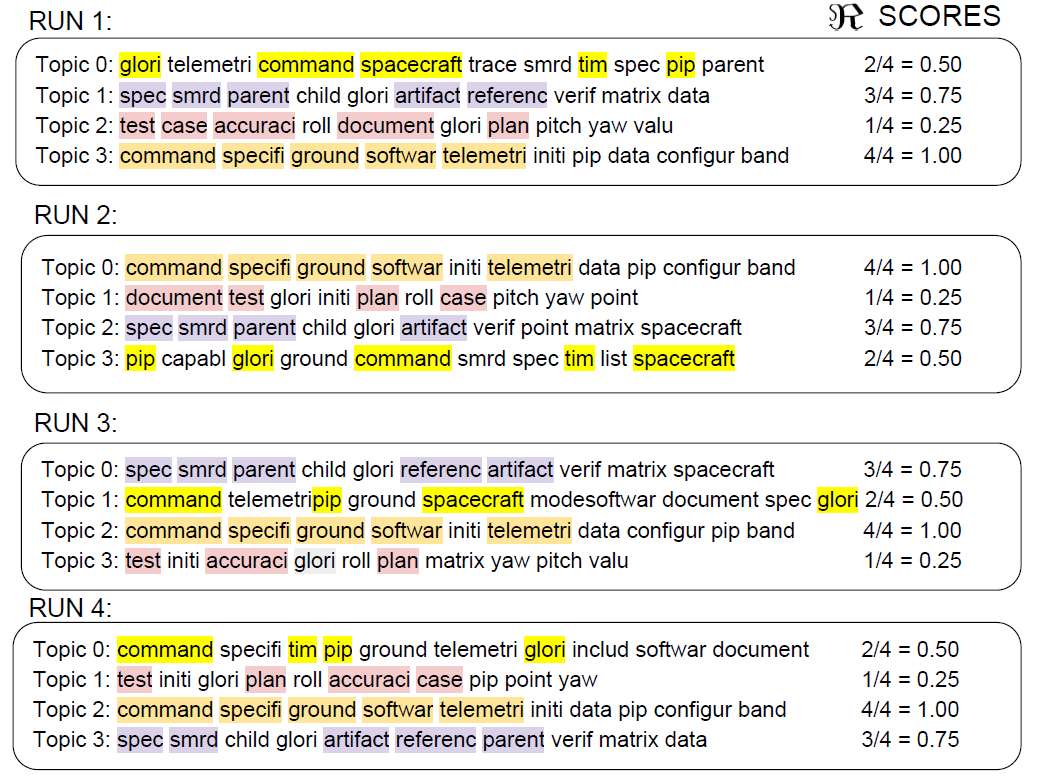
\includegraphics[width=13cm]{./fig/jaccard.png}
    \end{center}
  \caption{Example of topics overlap off size $n=5$ across multiple runs.}
  \label{fig:jaccard}
\end{figure*}


\subsection{Data Sets}
To answer our research questions, and to enable reproducibility of our results,
we use three open source datasets summarized in Table~\ref{tbl:dataset} and described
below. These 3 datasets are unrelated which solve different SE tasks. We wanted to make sure our LDADE is useful for atleast these 3 tasks. This puts emphasis on the importance of stability in LDA for any SE task. 

\textbf{PITS} is a text mining data set generated from NASA software project
and issue tracking system (PITS) reports~\cite{menzies2008improving, menzies2008automated}. This text discusses
bugs and changes found in big reports and  review patches.
Such issues are used
to manage quality assurance, to support communication
between developers. Topic modeling in PITS can be used
to identify the top topics which can
identify each severity separately. The dataset can be downloaded from the
PROMISE
repository~\cite{promiserepo}. Note that, this data comes from six different
NASA projects, which we label as PitsA, PitsB, etc.
    
 \textbf{Stackoverflow} is the flagship site of the Stack Exchange Network which
 features questions and answers on a wide range of topics in computer
 programming. There has been various studies done to find good topics on Stackoverflow for SE~\cite{barua2014developers,linares2013exploratory, allamanis2013and,rosen2016mobile}.
Topic modeling on Stackoverflow is useful for finding patterns in programmer knowledge.
 This data can be downloaded online\footnote{http://tiny.cc/SOProcess}. 
    
  \textbf{Citemap} contains titles and abstracts of 15121 papers from a
 database of 11 senior software engineering conferences from 1992-2016. Most of this data was
 obtained in the form of an SQL dump from the work of Vasilescu et
 al.~\cite{vasilescu2013historical} and some are collected by Mathew et al~\cite{mathew2016trends}. People have studied healthiness of software engineering conferences~\cite{vasilescu2014healthy}. This dataset is available on-line\footnote{https://github.com/ai-se/citemap/blob/master/citemap.csv}.

  For this study, all  datasets were preprocessed using the usual text mining filters~\cite{feldman2006j}:
\bi
\item
  Stop words removal using NLTK toolkit\footnote{http://www.nltk.org/book/ch02.html}~\cite{bird2006nltk} : ignore very common short words such as  ``and'' or ``the''.
\item
  Porter's stemming filter~\cite{Porter1980}: delete uninformative word endings; e.g. after performing stemming, all the following words would be rewritten
  to ``connect'': ``connection'', ``connections'',
``connective'',          
``connected'',
  ``connecting''.
\item
  Tf-idf feature selection: focus on the 5\% of words that occur frequently,
  but only in small numbers of documents. If a word occurs $w$ times
  and is found in $d$ documents  and there
  are $W,D$ total number of words and documents respectively, then tf-idf is scored
  as follows:
  \[
  \mathit{tfidf}(w,d)=   \frac{w}{W} *\log{\frac{D}{d}}\]
  \ei

  Table~\ref{tbl:dataset} shows the sizes of our data before and after pre-processing.
  These datasets are of different sizes and so are processed using different tools:
  \bi
\item PITS and Citemap is small enough to process on a single (four core) desktop machine
  using Scikit-Learn~\cite{pedregosa2011scikit} and Python.
  \item Stackoverflow is so large (7GB) that its  processing requires extra hardware support.
 This study used Spark and Mllib on a cluster of 45 nodes to
 reduce the runtime.
 \ei
  




\subsection{Similarity Scoring}
%YY this apra makes no sense
%% To evaluate the topics coherence or the cluster stability using LDA, there has
%% been number of evaluation measures proposed. There is a direct approach, by
%% asking people about topics, and an indirect approach by evaluating
%% \textit{pointwise mutual information (PMI)}~\cite{lau2014machine, o2015analysis}
%% between the topic words. PMI being an automatic method, we are not sure of exact
%% details of it which made us to not use this measure. We could not use direct
%% approach, due to resource limitation to ask an expert for the type of datasets
%% we used.
To evaluate topics coherence in LDA, there is a direct approach, by asking people about topics, and an indirect approach by evaluating \textit{pointwise mutual information (PMI)}~\cite{lau2014machine, o2015analysis} between the topic words. We could not use any of these criteria, as it requires experts to have domain knowledge. \textit{Perplexity} is  the inverse of the geometric mean per-word likelihood. The smaller the perplexity, the better (less uniform) is the LDA model. The usual trend is that as the value of perplexity drops, the number of topics should grow~\cite{koltcov2014latent}. Researchers caution that the value of perplexity doesn't remain constant with different topic size and with dictionary sizes~\cite{ zhao2015heuristic}. A lot depend on the code implementation of perplexity and the type of datasets used. Since, we are using different implementations of LDA across different platforms on various datasets, we are not using perplexity as evaluation measure.

There is well known measure, called \textit{Jaccard Similarity}~\cite{o2015analysis, galvis2013analysis}, for measuring similarity. But we modified the measure to do a cross-run similarity of topics. For this work, we assess topic model stability via the {\em median number overlaps of size $n$ words $\mathit{(size\_of\_topic)}$}, which we denote $\Re_n$.

%XXX  The magical number seven plus or minus two: some limits on our capacity for processing information.
%by: G. A. MILLER
%Psychological review, Vol. 63, No. 2. (March 1956), pp. 81-97  Key: citeulike:1089248
 


For this measurement, we first determine the maximum size of topics we will study. For that purpose,
we will study the case of $n \le 9$ (we use 9 as our maximum size since the cognitive
science literature tells us that $7\pm 2$ is a useful upper size for artifacts to be browsed by humans~\cite{miller1956magical}).


Next, for $1 \le n \le 9$, we will calculate the median size of the overlap,
computed as follows:
\bi
\item Let one {\em run} of our rig shuffle the order of the training data, then build topic models using the data;
  \item $m$ runs of our rig execute $m$ copies of one run, each time using a different random number seed,
\item We say topics are stable,
when there are $x$ occurrences of  $n$ terms appearing in all the topics seen in the $m$ runs.
\ei


For example, consider the topics shown in Figure~\ref{fig:jaccard}. These are generated via four {\em runs} of our system. In this hypothetical example, we will assume that the runs of
 Figure~\ref{fig:jaccard} were generated by an LDA suffering from topic instability.
For $n=5$, we note that Topic~0 of run1 scores $\frac{2}{4}=0.5$ since it shares 5 words with topics in only two out of four runs.
Repeating that calculation for the other run1 topics shows that:
\bi
\item Topic~1 of run1 scores $\frac{3}{4}=0.75$;
\item Topic~2 or run1 scores $\frac{1}{4}=0.25$;
\item Topic~3 of run1 scores $\frac{4}{4}=1$.
  \ei
  From this information, we can calculate
  $\Re_5$  (the
  {\em median number overlaps of size $n=5$ words}) as:
  \[
   \mathit{median}(0.5, 0.75, 0.25, 1) =0.625\]
  %YYY need an example of Fig5 here using the data of Figure4.
  Figure~\ref{fig:alln}
  shows the $\Re_n$ scores of 
  Figure~\ref{fig:jaccard} for $1 \le n \le 9$.  From this figure, we can see LDA topic instability
  since
  any report of the contents of a topic that uses more than three words per topic would be unreliable.

  \begin{figure}[!h]
  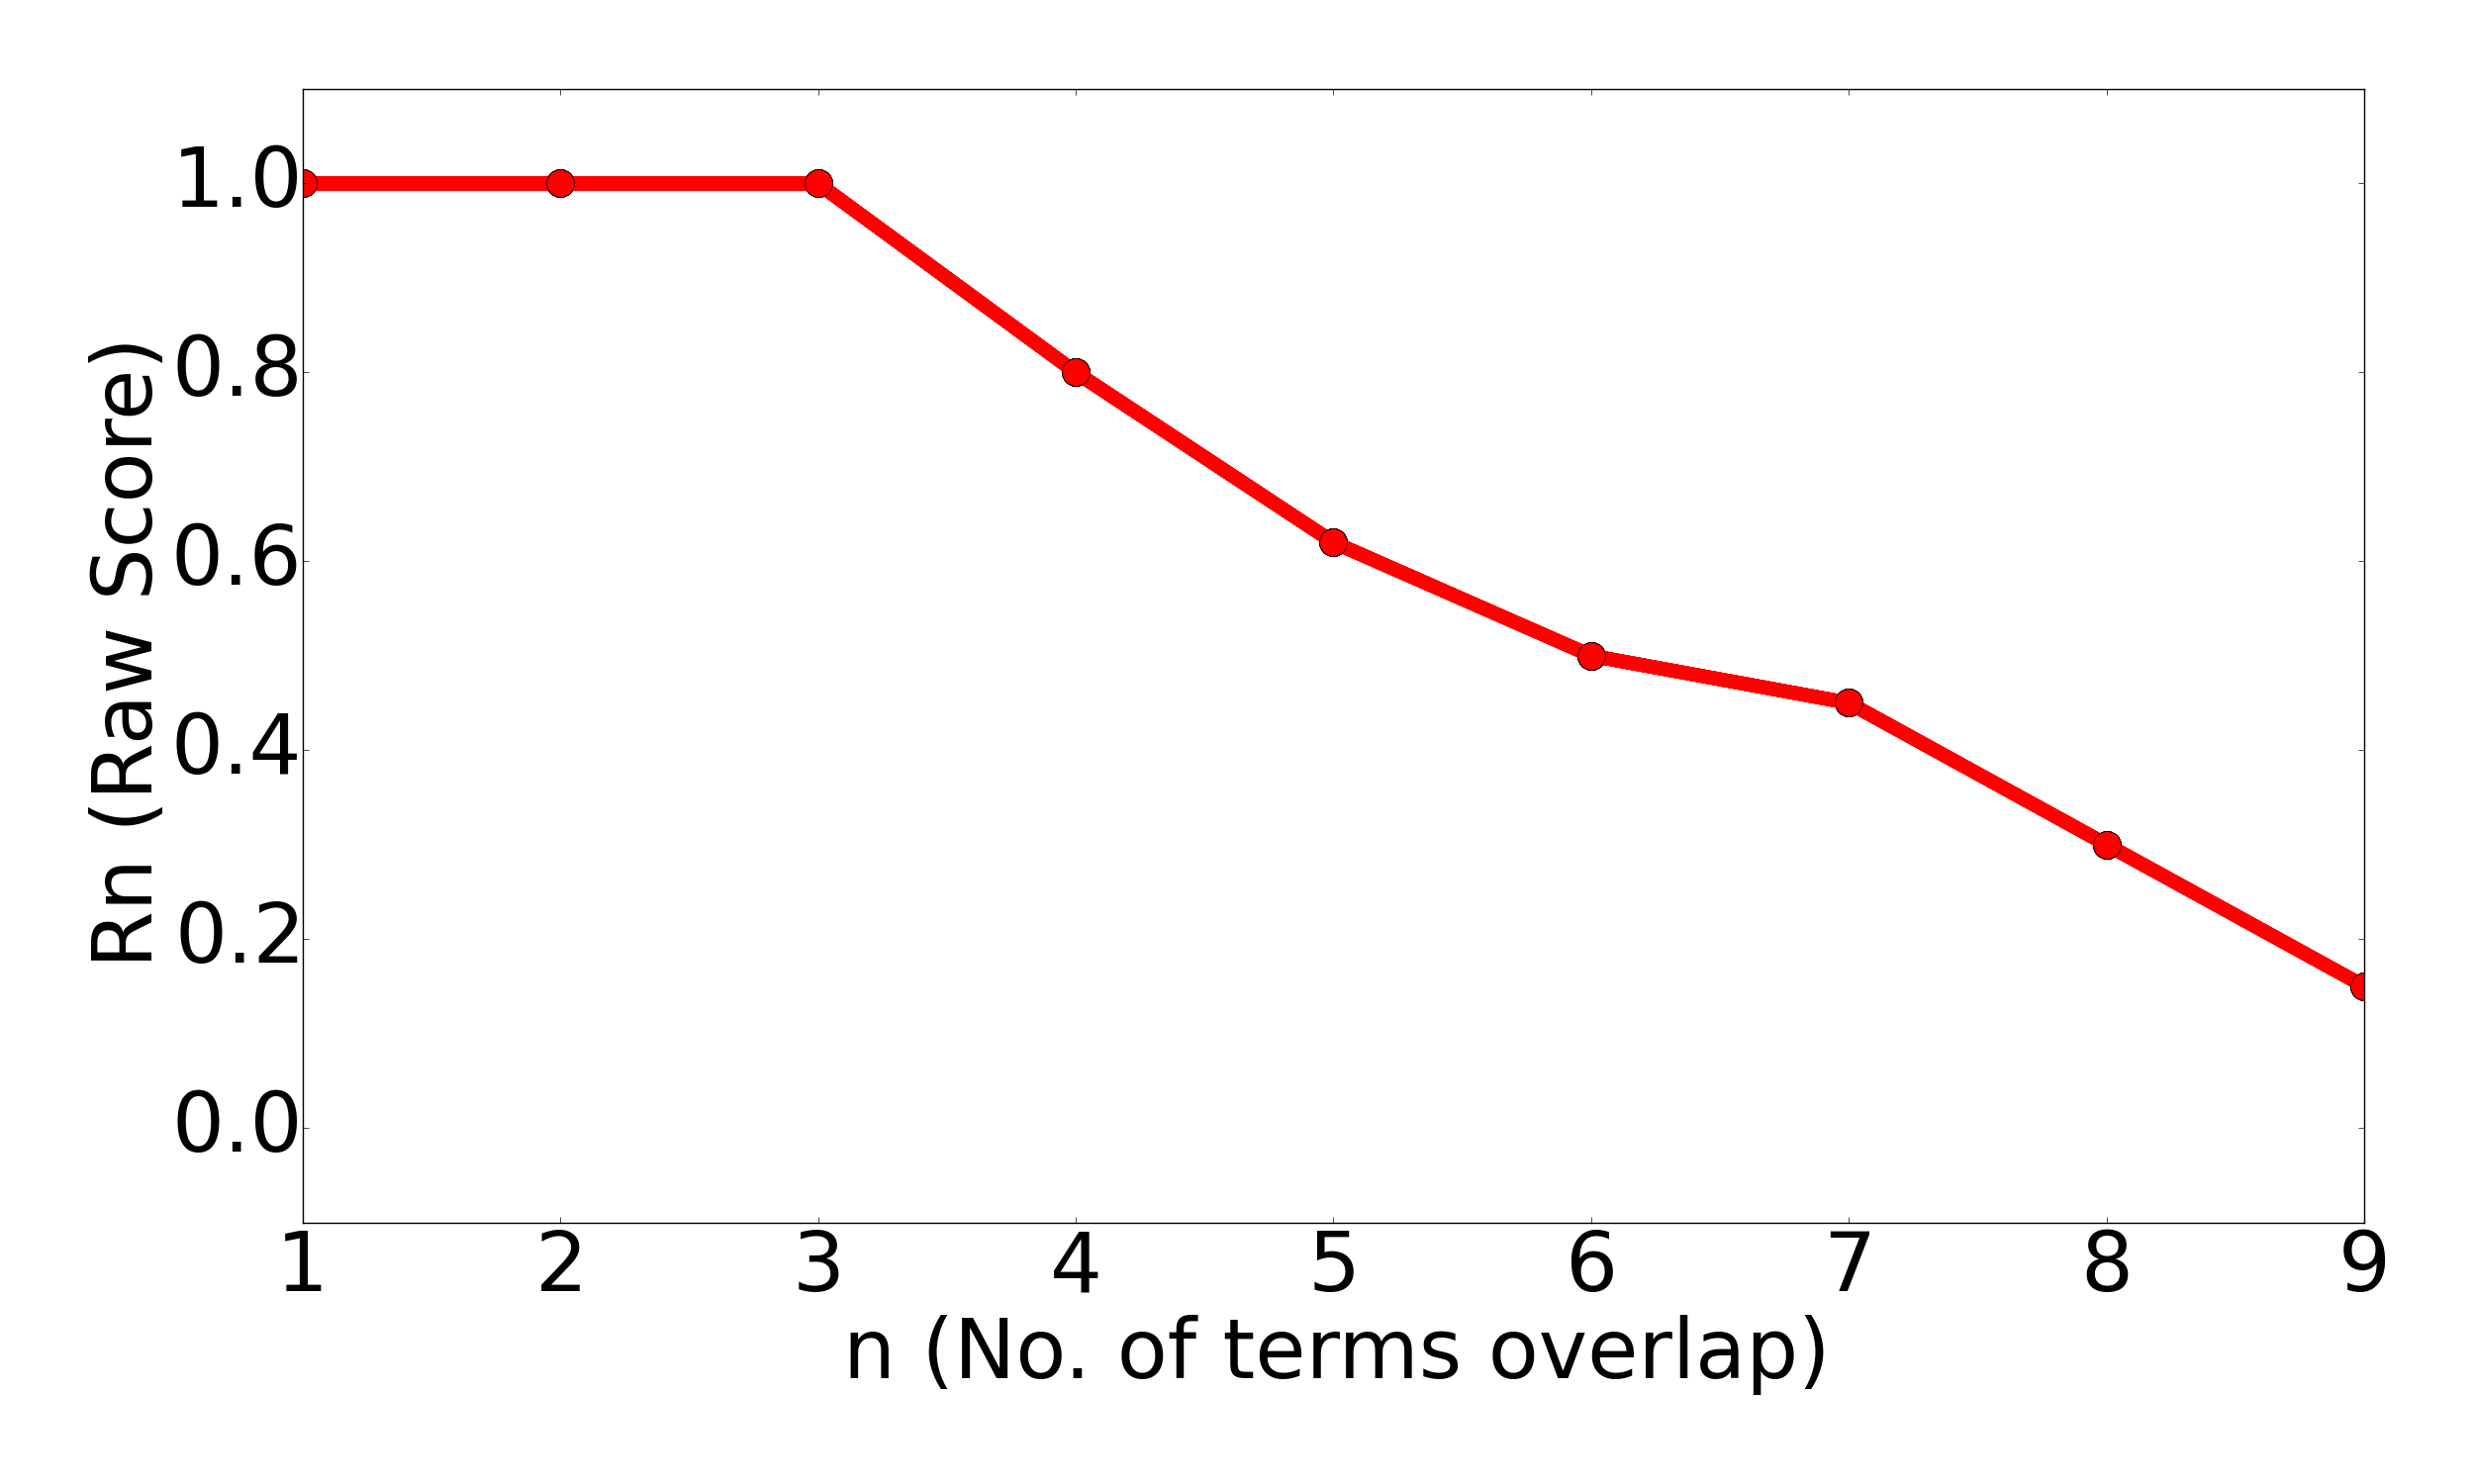
\includegraphics[width=\linewidth]{./fig/alln.png}
  \caption{$\Re_n$ scores of 
  Figure~\ref{fig:jaccard} for $1 \le n \le 9$}
  \label{fig:alln}
\end{figure}

 For the following analysis,
 %YYY do our graphs really use this terminology?
we distinguish between the \textbf{\textit{Raw  score}} and the \textbf{\textit{Delta  score}}:
 \bi
\item The two \textbf{\textit{Raw  scores}} are the $\Re_n$ median similarity scores seen {\em before} and {\em after} tuning LDA;
\item The \textbf{\textit{Delta score}} is the difference between the two
  \textbf{\textit{Raw scores}} (after tuning - before tuning).  \ei 
  The pseudocode for these calculations
  is shown in Algorithm 1 with the default set of parameters. In the following
  description, superscript numbers denote lines in the pseudocode. The data ordering is
  shuffled every time LDA is ran$^{5}$. Data is in the form of term frequency
  scores of each word per document. Shuffling is done in order to induce maximum
  variance among the ordering of data with  different runs of LDA. Topics$^{6}$ are a list of lists which
  contains topics from all the different runs. A stability score is evaluated on
  every 10 runs (Fixed), and this process is continued 10 (Fixed) times. At the end, the median
  score is selected as the untuned raw score ($\Re_n$ ) $^{3-11}$. Hence, the runtimes comes from $10 * 10$ evaluations of untuned experiment.

\makeatletter
\algrenewcommand\ALG@beginalgorithmic{\footnotesize}
\algrenewcommand\algorithmiccomment[2][\normalsize]{{#1\hfill\(\triangleright\) #2}}
\makeatother
\renewcommand{\algorithmicrequire}{\textbf{Input:}}
\renewcommand{\algorithmicensure}{\textbf{Output:}}
\begin{algorithm}
    %\scriptsize
    %\label{algo: untuned}
    
    \begin{algorithmic}[1]
    %\label{algo: untuned}
    \Require $Data$, $n$, $k$, $\alpha$, $\beta$ (Defaults) 
    \Ensure $Raw\_Score$    
    \Function{ldascore}{ $n$, $Data$}
        \State $Score \leftarrow \emptyset$
        \For{$j = 0$ to 10}
            \For{$i = 0$ to 10}
                \State $data \leftarrow$ \textbf{shuffle}($Data$)
                \State $Topics$.add(lda($k,\alpha,\beta$ ))
            \EndFor
            \State $Score$.add($Overlap$(Topics, $n$, $l[0]$))
        \EndFor
        \State $Raw\_Score \leftarrow $ median(Score)
        \State \textbf{return} $Raw\_Score$
    \EndFunction
    %\medskip
    \caption{Pseudocode for untuned LDA with Default Parameters}
    \end{algorithmic}
\end{algorithm}

\subsection{Tuning Topic Modeling with LDADE}
\label{sect:tuning}
LDADE is a combination of topic modeling (with LDA) and an optimizer (differential evolution, or DE) that adjusts
the parameters of LDA in order to optimize (i.e. maximize) similarity scores.

We choose to use DE after a literature search on search-based SE methods.
The literature mentions many optimizers: simulated
annealing~\cite{feather2002converging, menzies2007business}; various genetic
algorithms~\cite{goldberg1979complexity} augmented by techniques such as
DE (differential evolution~\cite{storn1997differential}), tabu search and scatter
search~\cite{glover1986general, beausoleil2006moss, molina2007sspmo,nebro2008abyss}; particle swarm optimization~\cite{pan2008particle}; numerous
decomposition approaches that use heuristics to decompose the total space into
small problems, then apply a response surface methods~\cite{krall2015gale, zuluaga2013active}.
Of these, we use DE for two reasons. Firstly, it has been proven useful in prior SE tuning
studies~\cite{fu2016tuning}. Secondly, our reading of the current literature is
that there are many advocates for differential evolution.

%\newpage
LDADE  adjusts the parameters of
Table~\ref{tb:tuned}. Most of these parameters were explained above. Apart from them, there are 2 different kinds of LDA implementations as well and they are:
\bi
\item VEM is the deterministic {\em variational EM} method that computes $\alpha$ and $\beta$ via
  expectation maximization~\cite{minka2002expectation}.
\item Gibbs sampling~\cite{wei2006lda, griffiths2004finding} is a Markov Chain Monte Carlo algorithm, which is an approximate stochastic process for computing and updating $\alpha$ and $\beta$.
  Topic modeling researchers in SE have argued that Gibbs leads to stabler models~\cite{layman16a,layman2016topic} (a claim which we test, below).
  \ei

We manually run with these other inference techniques according to different implementations across different platforms. We need to make sure that these instabilities do not hold for just 1 inference technique, or 1 implementation or on 1 platform.

\begin{table}[!htbp]
    \begin{center}
\scriptsize
\begin{tabular}{|c|c|c|p{3.5cm}|}
        \hline 
        \textbf{Parameters} & \textbf{Defaults} & \textbf{Tuning Range} & \textbf{Description}\\
        \hline
        $k$ & 10 & [10,100] & Number of topics or cluster size \\ 
        \hline
       $\alpha$ & None & [0,1] & Prior of document topic distribution. This is called alpha \\ 
        \hline
        $\beta$ & None & [0,1] & Prior of topic word distribution. This is called  beta \\

        \hline
\end{tabular}

\end{center}
\caption{List of parameters tuned by this paper}
\label{tb:tuned}
\end{table}

Algorithm 2 shows LDADE's version of DE.  DE evolves a \textit{NewGeneration} of
candidates from a current Population.   Each candidate solution in the Population is a pair of
(Tunings, Scores). Tunings are selected from Table \ref{tb:tuned} and scores
come similarly from Algorithm 1$^{3-11}$. Note that there is not any outer loop$^{3}$: in Algorithm 2, LDA is only run as one rig$^{11 \& 12}$. Here, the runtimes comes from $\mathit{iter} * np * 10$ evaluations of tuned experiment.

The main loop of DE$^{9}$ runs over the \textit{Population}, replacing old items with new Candidates (if new candidate is better).
DE generates \textit{new Candidates} via 
extrapolating$^{23}$ between current solutions in the frontier. Three solutions $a$, $b$ and $c$ are
selected at random. For each tuning parameter i, at some probability \textit{cr}, we
replace the old tuning $x_i$ with $y_i$. For booleans, we use $y_i = x_i$ (see
line 31). For numerics, $y_i = a_i + f \times (b_i - c_i)$ where $f$ is a
parameter controlling crossover. The trim function$^{33}$ limits the new value
to the legal range min..max of that parameter.

\renewcommand{\algorithmicrequire}{\textbf{Input:}}
\renewcommand{\algorithmicensure}{\textbf{Output:}}
\begin{algorithm}
  
    \begin{algorithmic}[1]
    \Require $np=10$, $f=0.7$, $cr=0.3$, $iter=3$, Goal $\in$ Finding maximum score
    \Ensure $Raw\_Score, final\_generation$
    \Function{DE}{$np,f,cr,iter, Goal$}
        \State  $Cur\_Gen \leftarrow \emptyset$
        \State $Population \leftarrow $InitializePopulation(np)
        \For{$i = 0$ to $np-1$}
            \State $Cur\_Gen$.add($Population$[i],ldascore($Population$[i],$n$,$Data$)
        \EndFor
        \For{$i = 0$ to $iter$}
            \State $NewGeneration \leftarrow \emptyset$
            \For{$j = 0$ to $np-1$}
                \State $S_i \leftarrow $Extrapolate($Population$[j],Population,cr,f,np)
                \If{ldascore($S_i$) $\geq$ $Cur\_Gen$[j][1]}
                    \State $NewGeneration$.add($S_i$,ldascore($S_i$,$n$, $Data$))
                \Else
                    \State $NewGeneration$.add($Cur\_Gen$[j])
                \EndIf
            
            \EndFor
            \State  $Cur\_Gen \leftarrow NewGeneration$
        \EndFor
        \State $Raw\_Score \leftarrow$ GetBestSolution($Cur\_Gen$)
        \State  $final\_generation \leftarrow Cur\_Gen$
        \State \textbf{return} $Raw\_Score, final\_generation$
    \EndFunction

    \Function{Extrapolate}{$old, pop, cr, f,np$}
        \State $a,b,c \leftarrow threeOthers$(pop, old)
        \State $newf \leftarrow \emptyset$
        \For{$i = 0$ to $np-1$}
            \If{$cr \leq$ random()}
                \State $newf$.add($old[i]$)
            \Else
                \If{typeof($old$[i])$ ==$ bool then}
                    \State $newf$.add(not $old[i]$)
                \Else 
                    \State $newf$.add(trim(i,($a$[i]+$f\ast$($b$[i] $-$ $c$[i]))))
                \EndIf
            \EndIf
        \EndFor
        \State \textbf{return} $newf$ 
    \EndFunction
    \caption{Pseudocode for DE with a constant number of iterations}
    \end{algorithmic}
\end{algorithm}

The loop invariant of DE is that, after the zero-th iteration$^7$, the \textit{Population}
contains examples that are better than at least one other candidate.
As the looping progresses, the \textit{Population} is full of increasingly more valuable solutions
which, in turn, also improve the candidates, which are Extrapolated from the Population.
Hence, Vesterstrom et al.~\cite{vesterstrom2004comparative} found DE to be
competitive with particle swarm optimization and other GAs.

Note that DEs have been
applied before for parameter tuning (e.g. see~\cite{omran2005differential,chiha2012tuning, fu2016tuning} ) but this is the first time they have been
applied to tune LDA to increase stability.

\section{Experimentation}\label{sect:results}

In this section,
 any result from the smaller data sets (Pits and Citemap) come
from Python implementation based on Scikit-Learn running on a 4 GB ram machine (Linux, Macintosh).
Also,
  any results from the larger data (Stackoverflow) comes from a Scala implementation
  based on Mllib~\cite{meng2016mllib} running on a 45 node Spark system (8 cores per node).
  
  Note that, for the RQ3, there are some intricate details with classification results. After tuning (Goal is still to maximize the $\Re_n$ score) and finding the optimal `K', we trained a Linear Kernel SVM classifier using document topic distributions as features just like used by Blei et al~\cite{blei2003latent}.


\subsection{\textbf{RQ1: Are the default settings of LDA incorrect?}}\label{sect:unstable}


This first research question checks the core premise of this article-- that changes
in the order of training data dramatically affects the topics learned via LDA.
Note that if this is {\em not true}, then there would be no value-added to this paper. 


 
\begin{figure}[!b]
  \begin{center}
    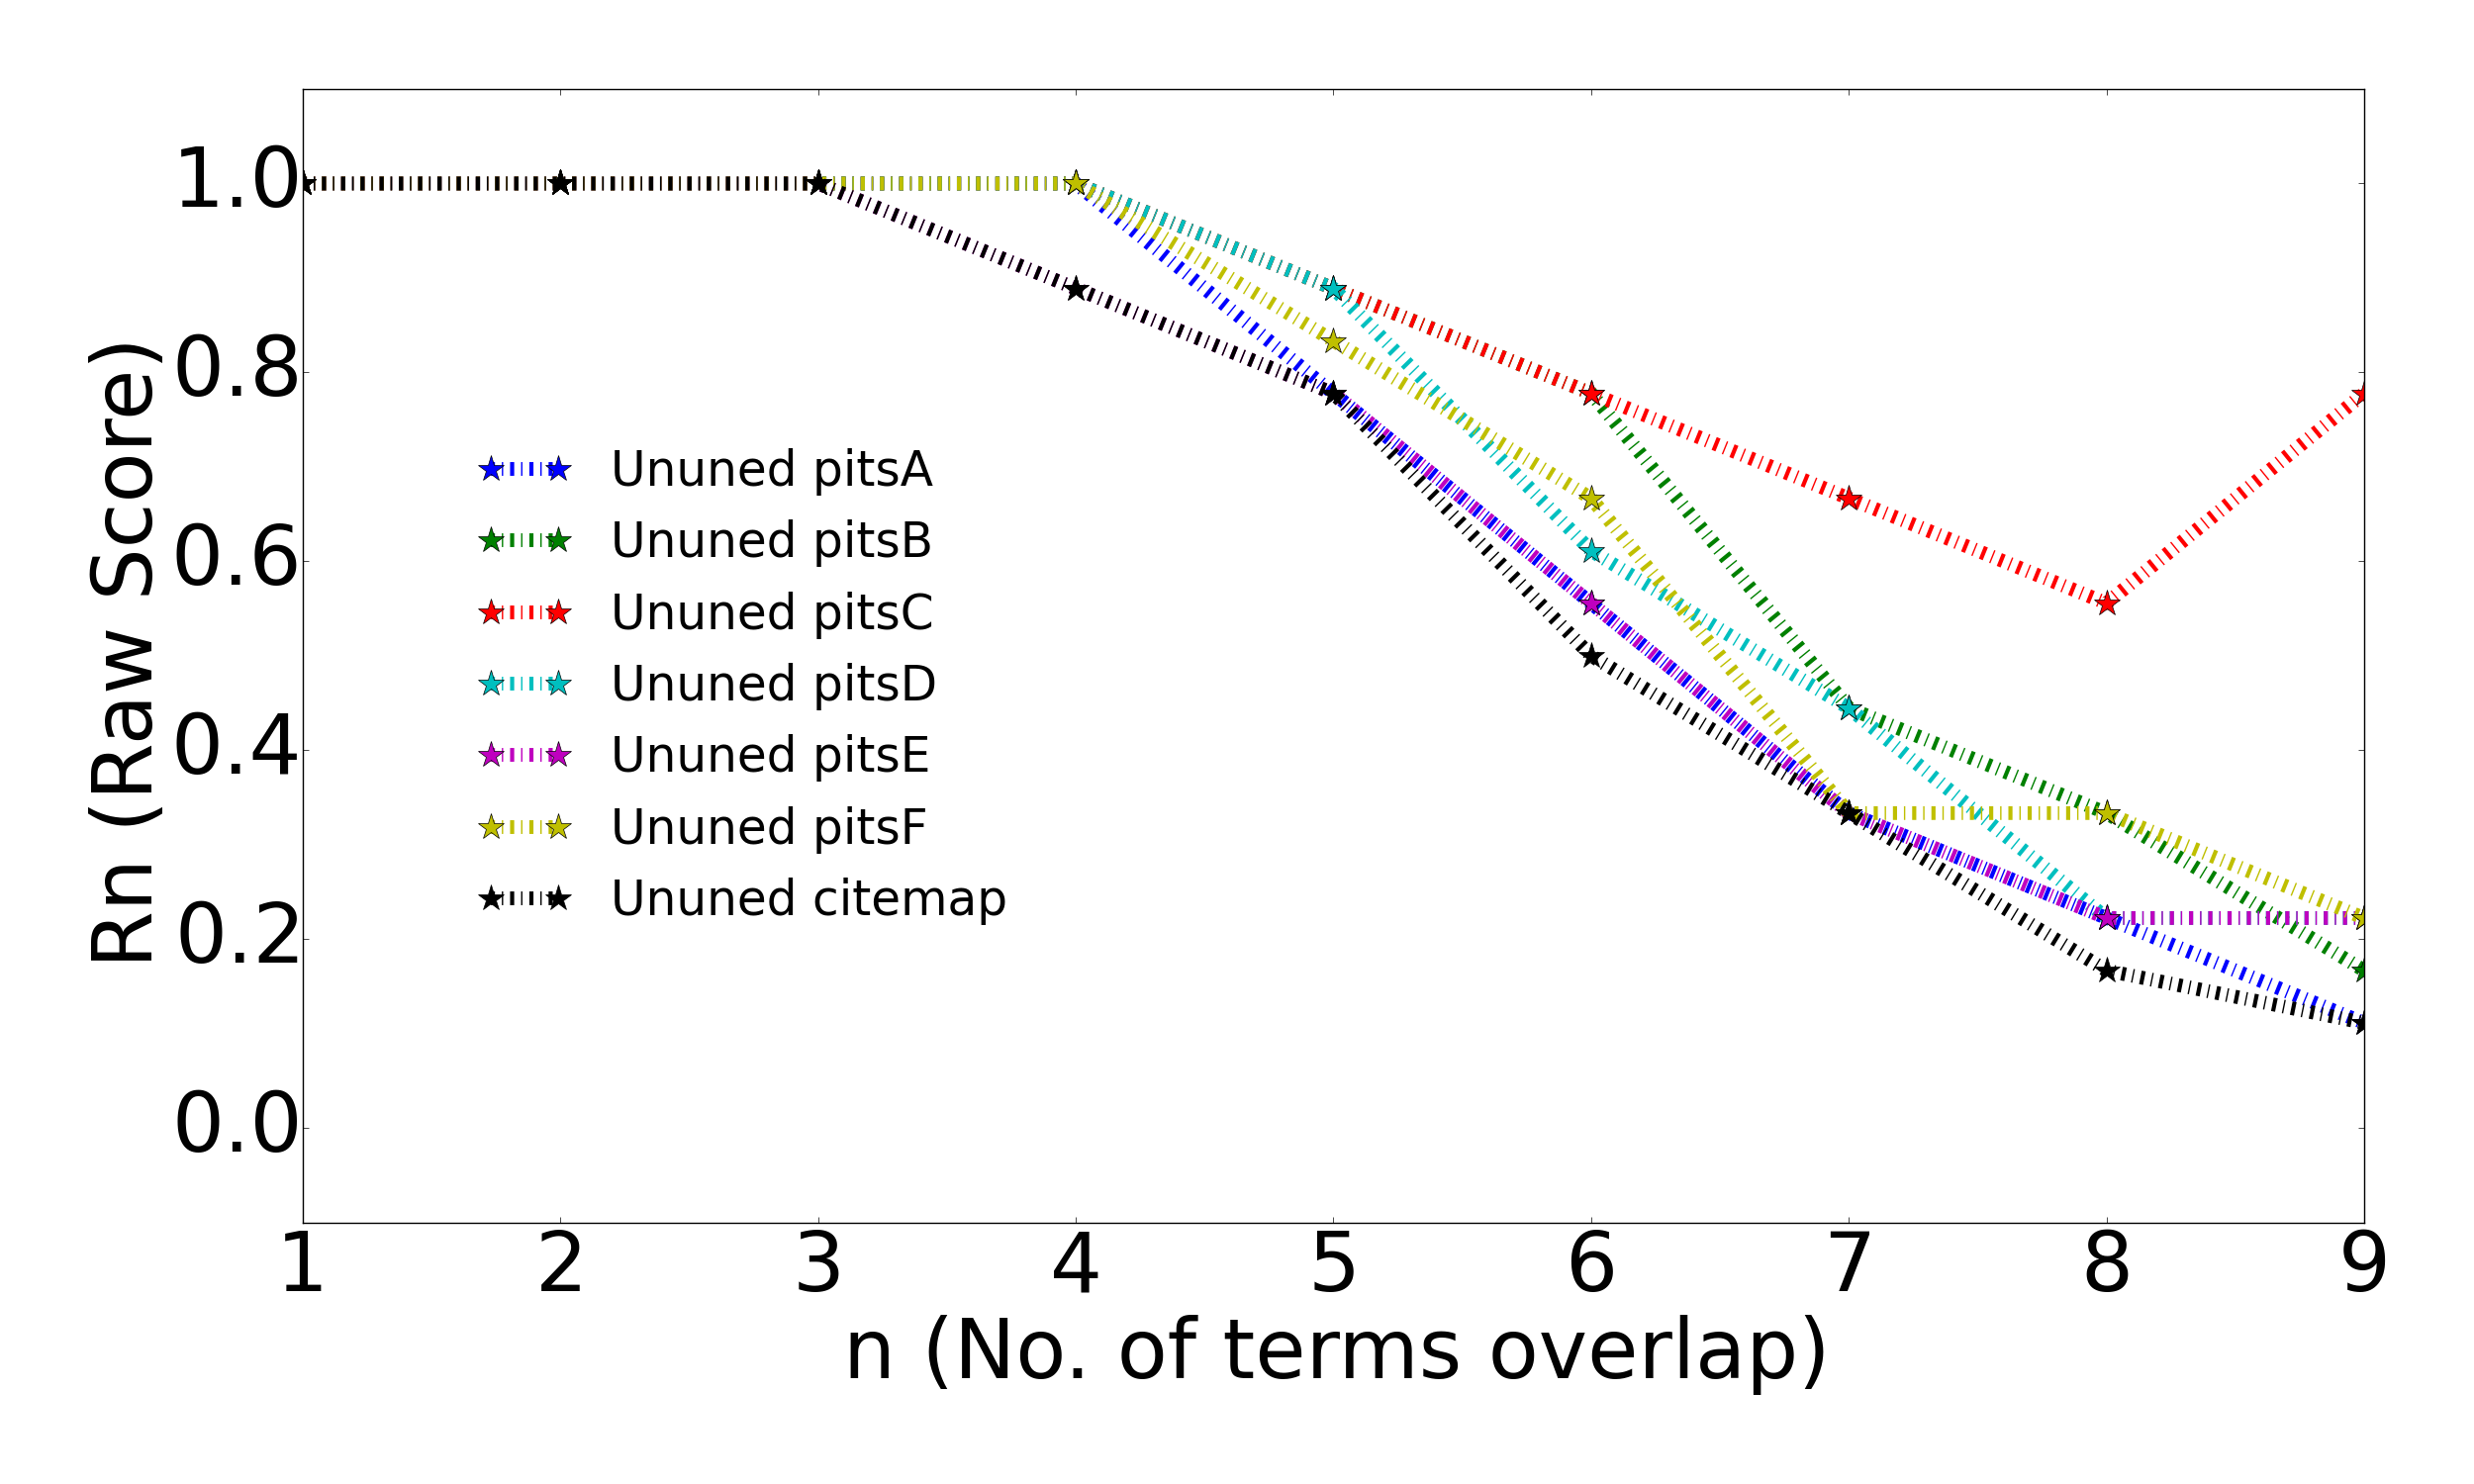
\includegraphics[width=\linewidth]{./fig/Vem_untuned.png}
    \end{center}
  \caption{{\em Before} tuning: uses LDA's default parameters}\label{fig:delta11}  
\end{figure}
\begin{figure}[!b]
        \begin{center}
        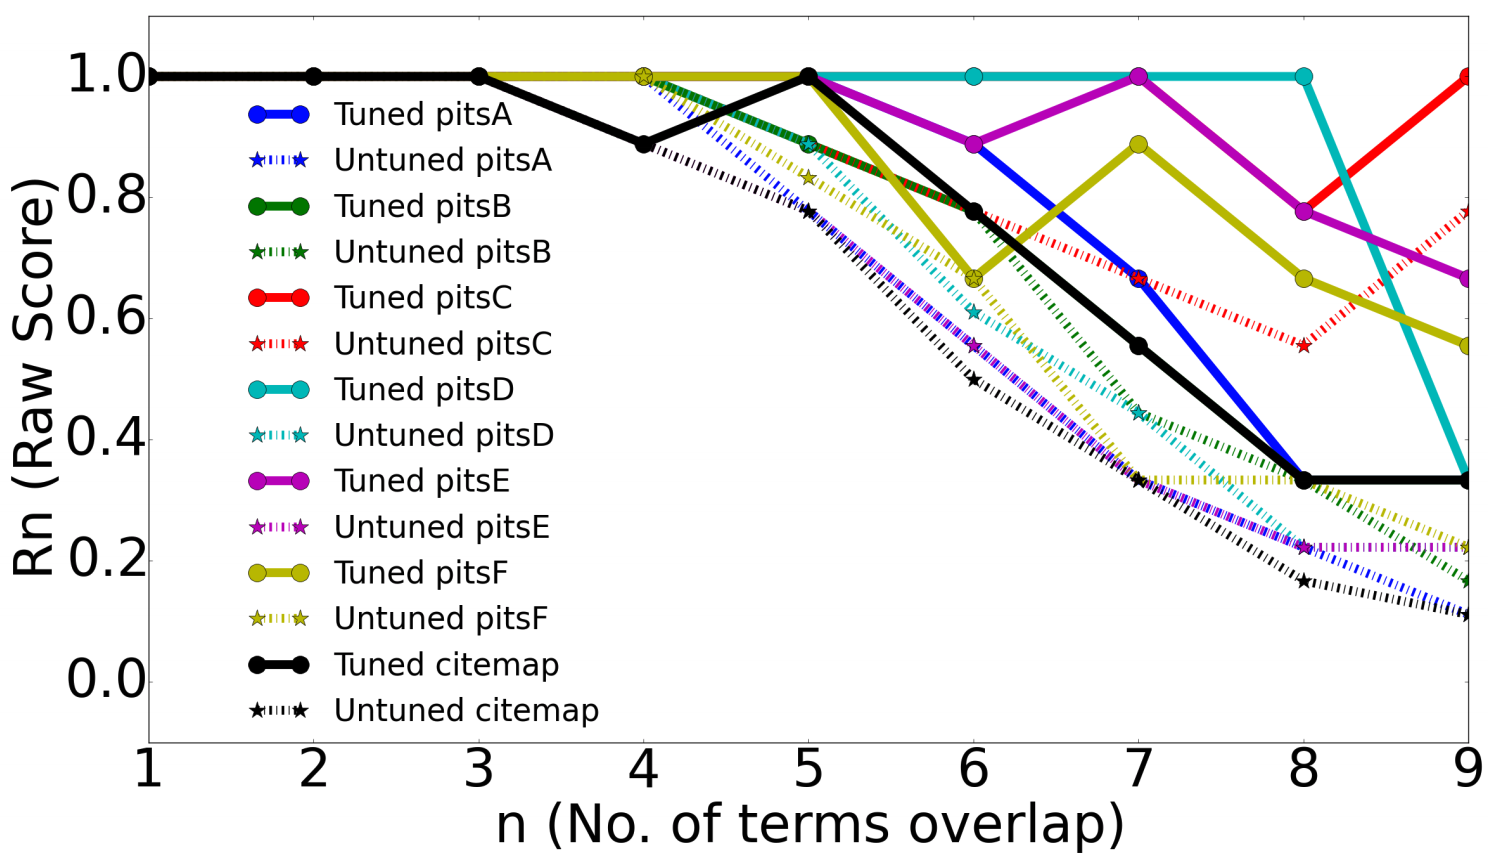
\includegraphics[width=0.9\linewidth]{./fig/raw_graph.png}
  \footnotesize{{\bf Figure~\ref{fig:delta}a:}  {\em After} tuning: uses parameters learned by DE.}

        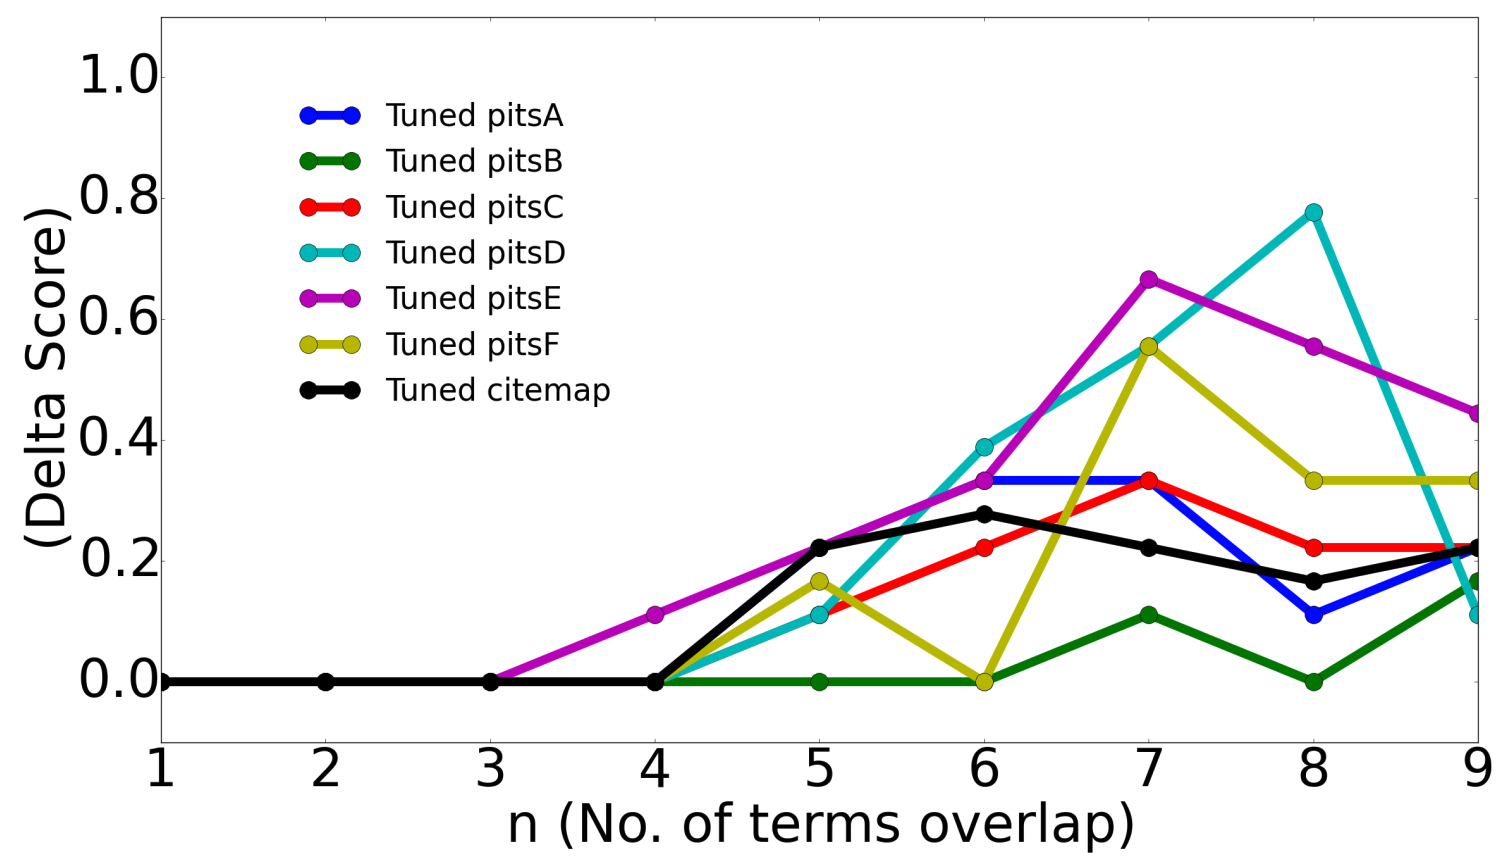
\includegraphics[width=0.9\linewidth]{./fig/tuned_delta_vem.png}
  \footnotesize{{\bf Figure~\ref{fig:delta}b:}  {\em Delta = After - Before}.}
  \end{center}
    \caption{{\bf RQ1, RQ2} stability results over ten repeated runs. In these figures, {\em larger} numbers
    are {\em better}.}\label{fig:delta}
\end{figure}

\begin{figure}[!b]
  \begin{center}
    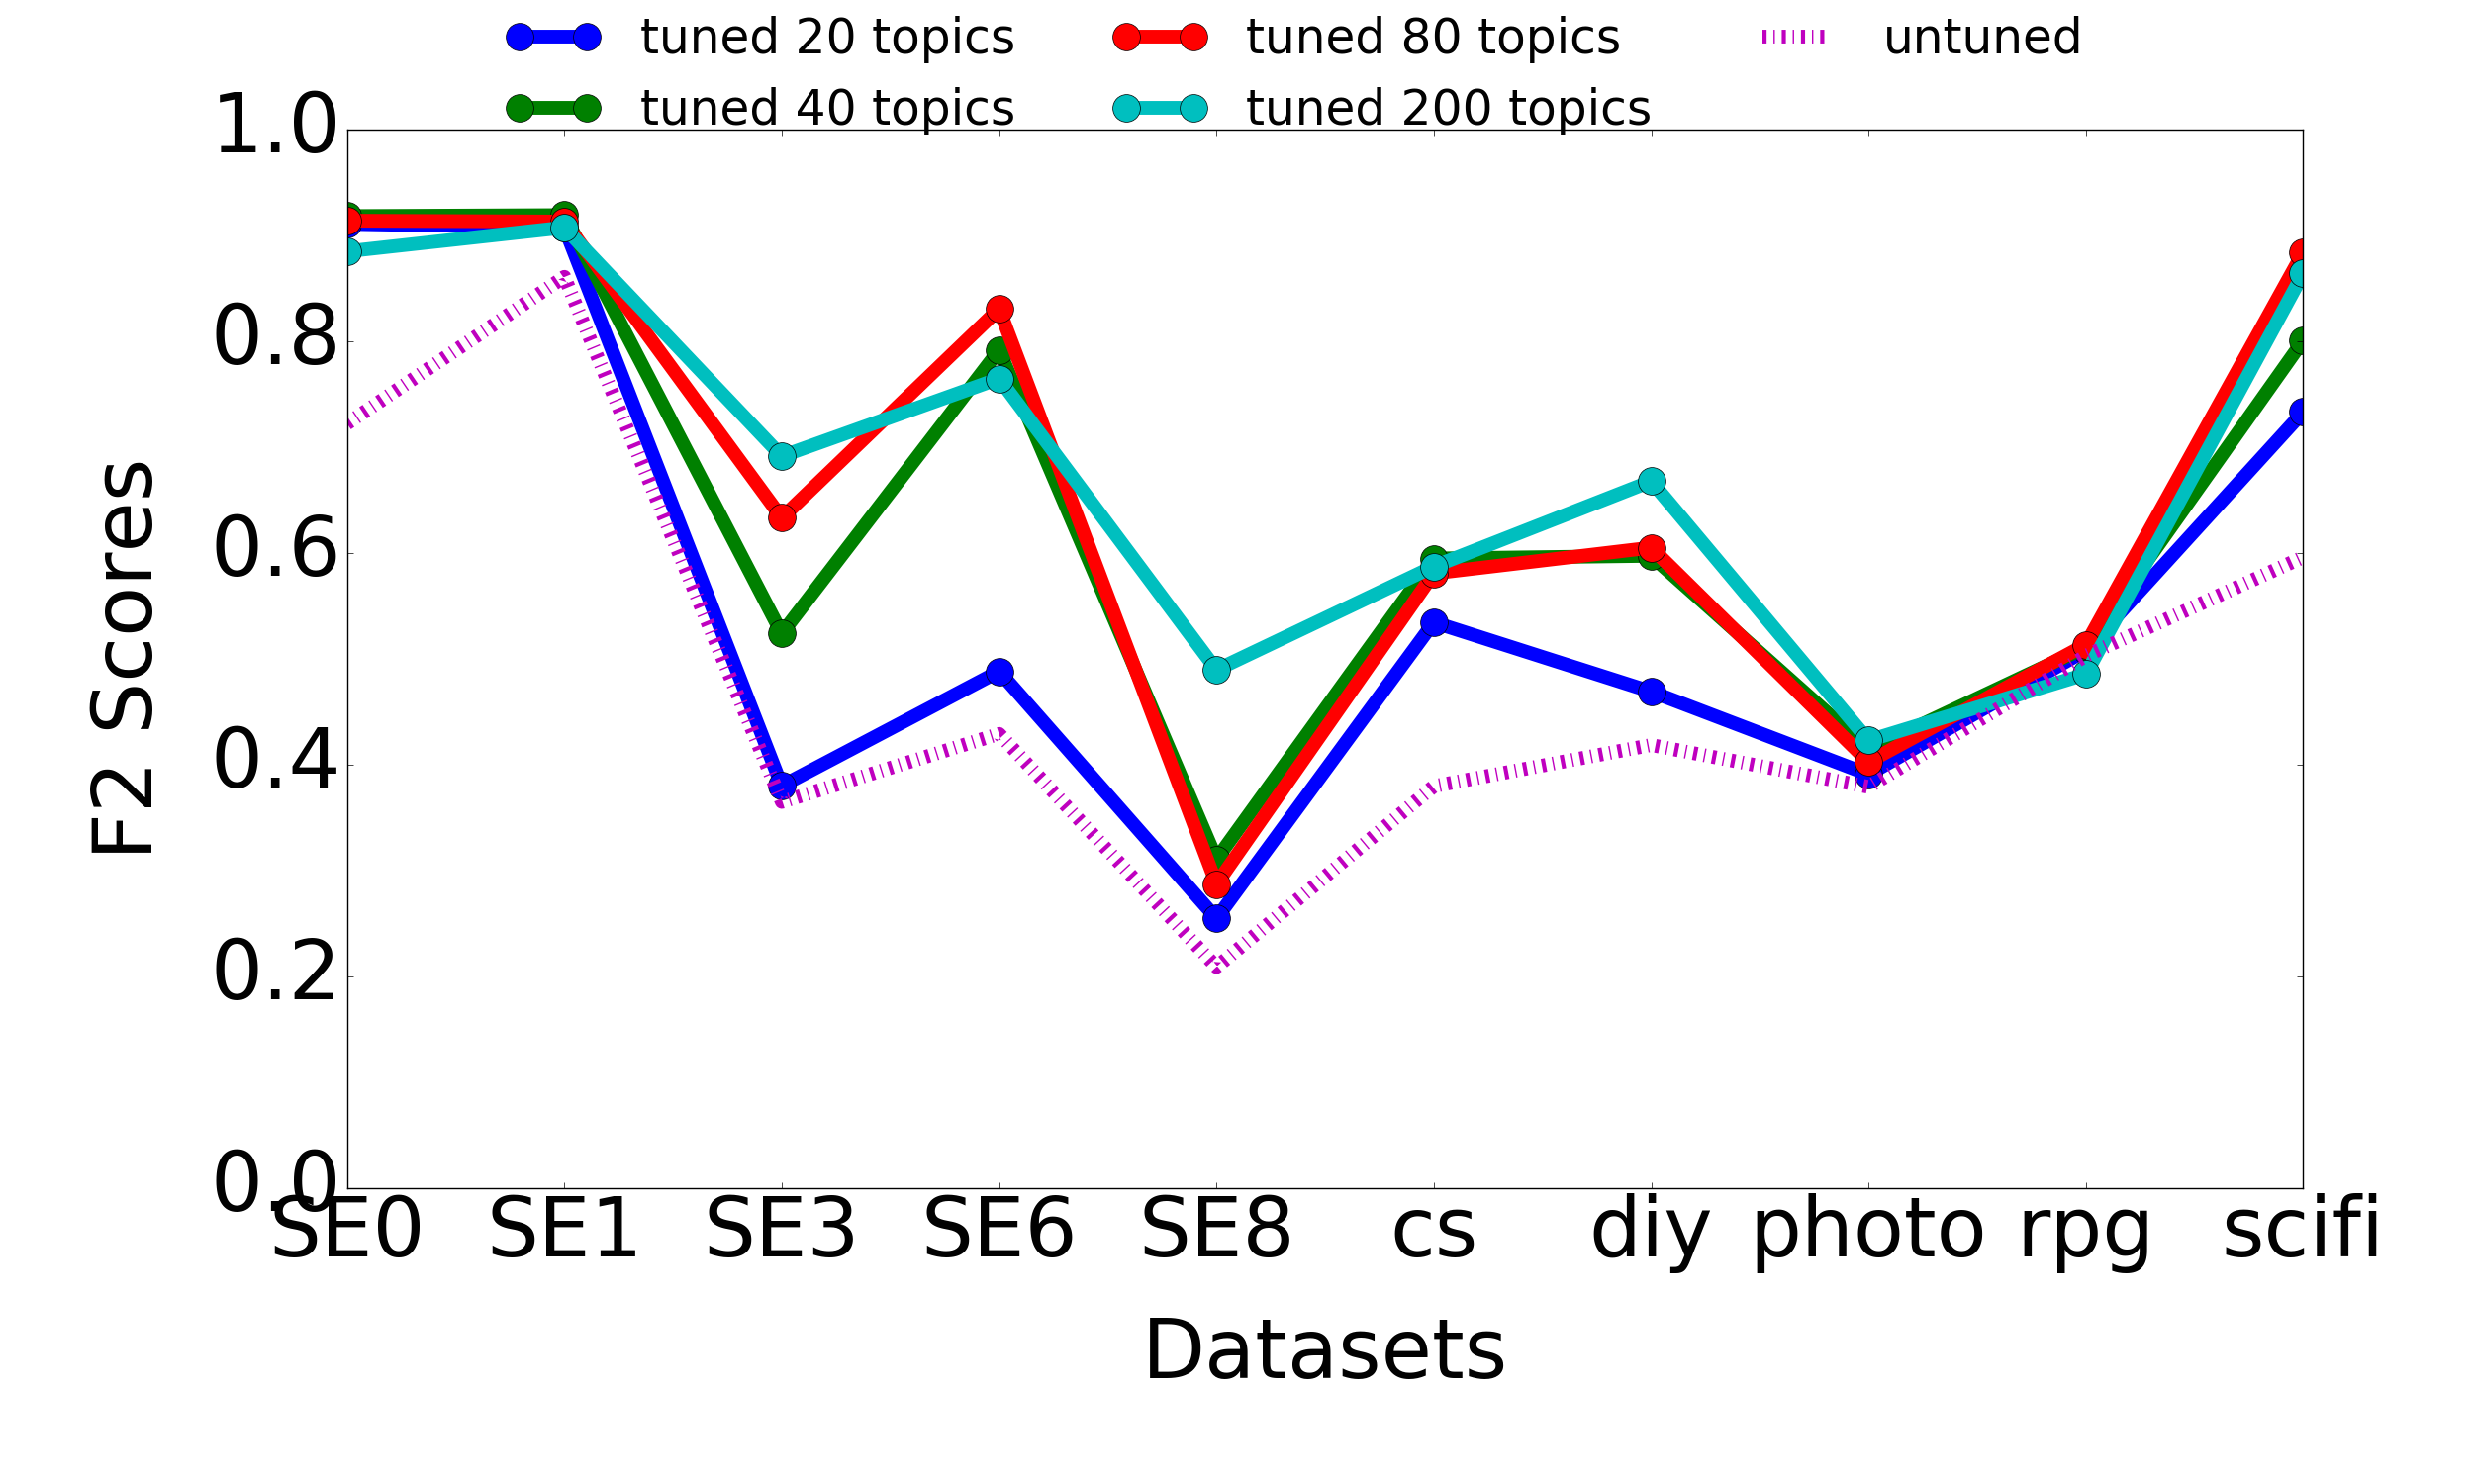
\includegraphics[width=\linewidth]{./fig/classification.png}
    \end{center}
  \caption{Tuning and Untuned results for Classification SE Task}\label{fig:class}  
\end{figure}

\begin{figure*}[!t]
    \centering
    \begin{minipage}{.33\textwidth}
        \captionsetup{justification=centering,singlelinecheck=off}
        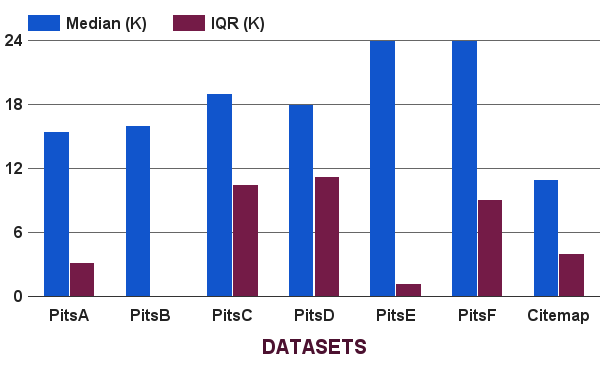
\includegraphics[width=\linewidth]{./fig/Parameters_variation_k.png}
        \caption{Datasets vs Parameter (k) variation}
        \label{RQ3:k}
    \end{minipage}%
    \begin{minipage}{.33\textwidth}
        \captionsetup{labelsep=space,justification=centering,singlelinecheck=off}
        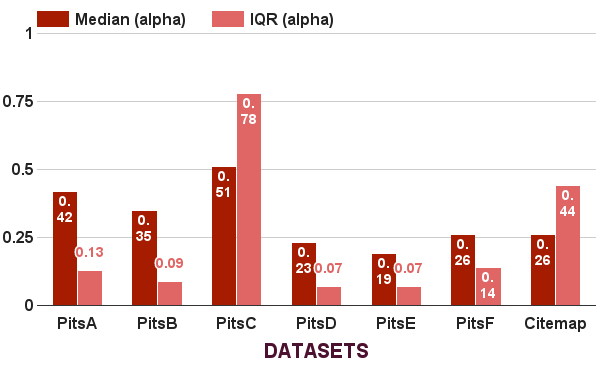
\includegraphics[width=\linewidth]{./fig/Parameters_variation_a.png}
        \caption{Datasets vs Parameter ($\alpha$) variation}
        \label{RQ3:a}
    \end{minipage}
    \begin{minipage}{.33\textwidth}
        \captionsetup{labelsep=space,justification=centering,singlelinecheck=off}
        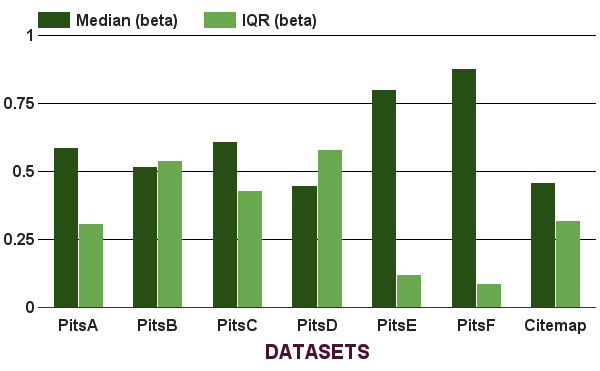
\includegraphics[width=\linewidth]{./fig/Parameters_variation_b.png}
        \caption{Datasets vs Parameter ($\beta$) variation}
        \label{RQ3:b}
    \end{minipage}
\end{figure*}

Figure~\ref{fig:delta11}   plots $n$ vs $\Re_n$ for untuned  LDA.
Note that the  stability collapses the most after $n=5$ words. This means
  that any report of LDA topics that uses more than five words per topic will
  be changed, just by changing the order of the inputs. This is a significant result
  since the standard advice in the LDA papers~\cite{panichella2013effectively, lukins2010bug}
  is to report the top 10 words per topic. As shown in Figure~\ref{fig:delta}a, it would
  be rare that any such 10 word topic would be found across multiple runs.
 \begin{lesson}
  Using the default settings of LDA for SE data can lead to systematic errors due to topic
  modeling instability. 
\end{lesson}


\subsection{\textbf{RQ2: Does LDADE improve the stability scores?}}\label{sect:stable}

 Figure~\ref{fig:delta}a and Figure~\ref{fig:delta}b shows the stability improvement
 generated by tuning.
   Tuning never
  has any negative effect (reduces stability) and often has a large positive effect--
  particular  after 5 terms overlap.
   The largest improvement  we
   was  in PitsD dataset which for up to 8 terms overlap was 100\% (i.e. was always
   found in all runs).
   Overall, after reporting topics of up to 7 words, in the majority case (66\%),
  those topics can be found in models generated using different input orderings.
  Accordingly, our answer to {\bf RQ2} is:

\begin{lesson}
For stable clusters, tuning is strongly recommended for future LDA studies. $\alpha$ and $\beta$ matter the most for getting good clusters.
\end{lesson}

\subsection{\textbf{RQ3:Does LDADE improve text mining classification accuracy?}}\label{sect:rq3} 

We studied some other StackExchange websites data dump for classification results which were generated by Krishna et al \cite{krishna2016bigse}. These datasets are categorized into binary labels saying which documents are relevant and non relevant. The goal of our DE was still to maximize the $\Re_n$ score. It shouldn't be confused with maximizing some other accuracy goals. After finding the optimal `K', we trained a Linear Kernel SVM classifier using document topic distributions just like used by Blei et al~\cite{blei2003latent}.

In Figure \ref{fig:class}, the x-axis represents different datasets as generated. Y-axis represents the F2 score
(from \eq{f}) which weights recall higher than precision~\cite{powers2011evaluation}. One legend called as ``untuned'' uses default parameters with $k=10$. Other legends in the graph show tuning of $k$ for 20, 40, 80 and 200 by keeping $\alpha$ and $\beta$ fixed. There is about 20\% minimum improvement over the untuned results.

\noindent
Hence, we say:

\begin{lesson}
For any SE classification task, tuning is again highly recommended. And $k$ matters the most for a good classification accuracy.
\end{lesson}

\subsection{\textbf{RQ4: Do different data sets
      need different configurations to make LDA stable?}}\label{sect:diff}

Figures \ref{RQ3:k}, \ref{RQ3:a}, and \ref{RQ3:b} show the results of tuning for word overlap of $n=5$.
On display in each set of vertical bars are
the median values generated across 10 tunings.
Also, shown are
the inter-quartile range (IQR) of those tunings (the IQR is the 75th-25th percentile values and is a non-parametric measure of variation
around the median value). Note that in Figure \ref{RQ3:k}, IQR=0 for  PitsB dataset where tuning
          always converged on the same final value.

  These figures
show how tuning selects the different ranges  of
parameters. 
Some of the above numbers are far from the standard values; e.g. Garousi et al.~\cite{garousi2016citations} recommend using $k=67$ topics
yet in our data sets, best results were seen using $k \le 24$.
Clearly:

\begin{lesson}
  Do not  reuse tunings suggested by other researchers from other data sets.
  Instead, always re-tune for all new data.
\end{lesson}
%Our results found out to be quite consistent and all our above research questions results hold valid in these scenarios as well. As to more specific threats to validity, one issue might be that our conclusions on ``LDA'' are really quirks of a specific implementation.

\subsection{\textbf{RQ5}: \textbf{Are our findings consistent using different kinds of LDA or with different implementations?}}

To validate this research question, it was insightful to compare our results with: the Pits and Citemap results, executed in Scikit-Learn and Python running on a desktop machine as well as the Stackoverflow data set executed in Scala using Mllib running on a Spark cluster.

\begin{figure}[!b]
  \captionsetup{justification=centering}
  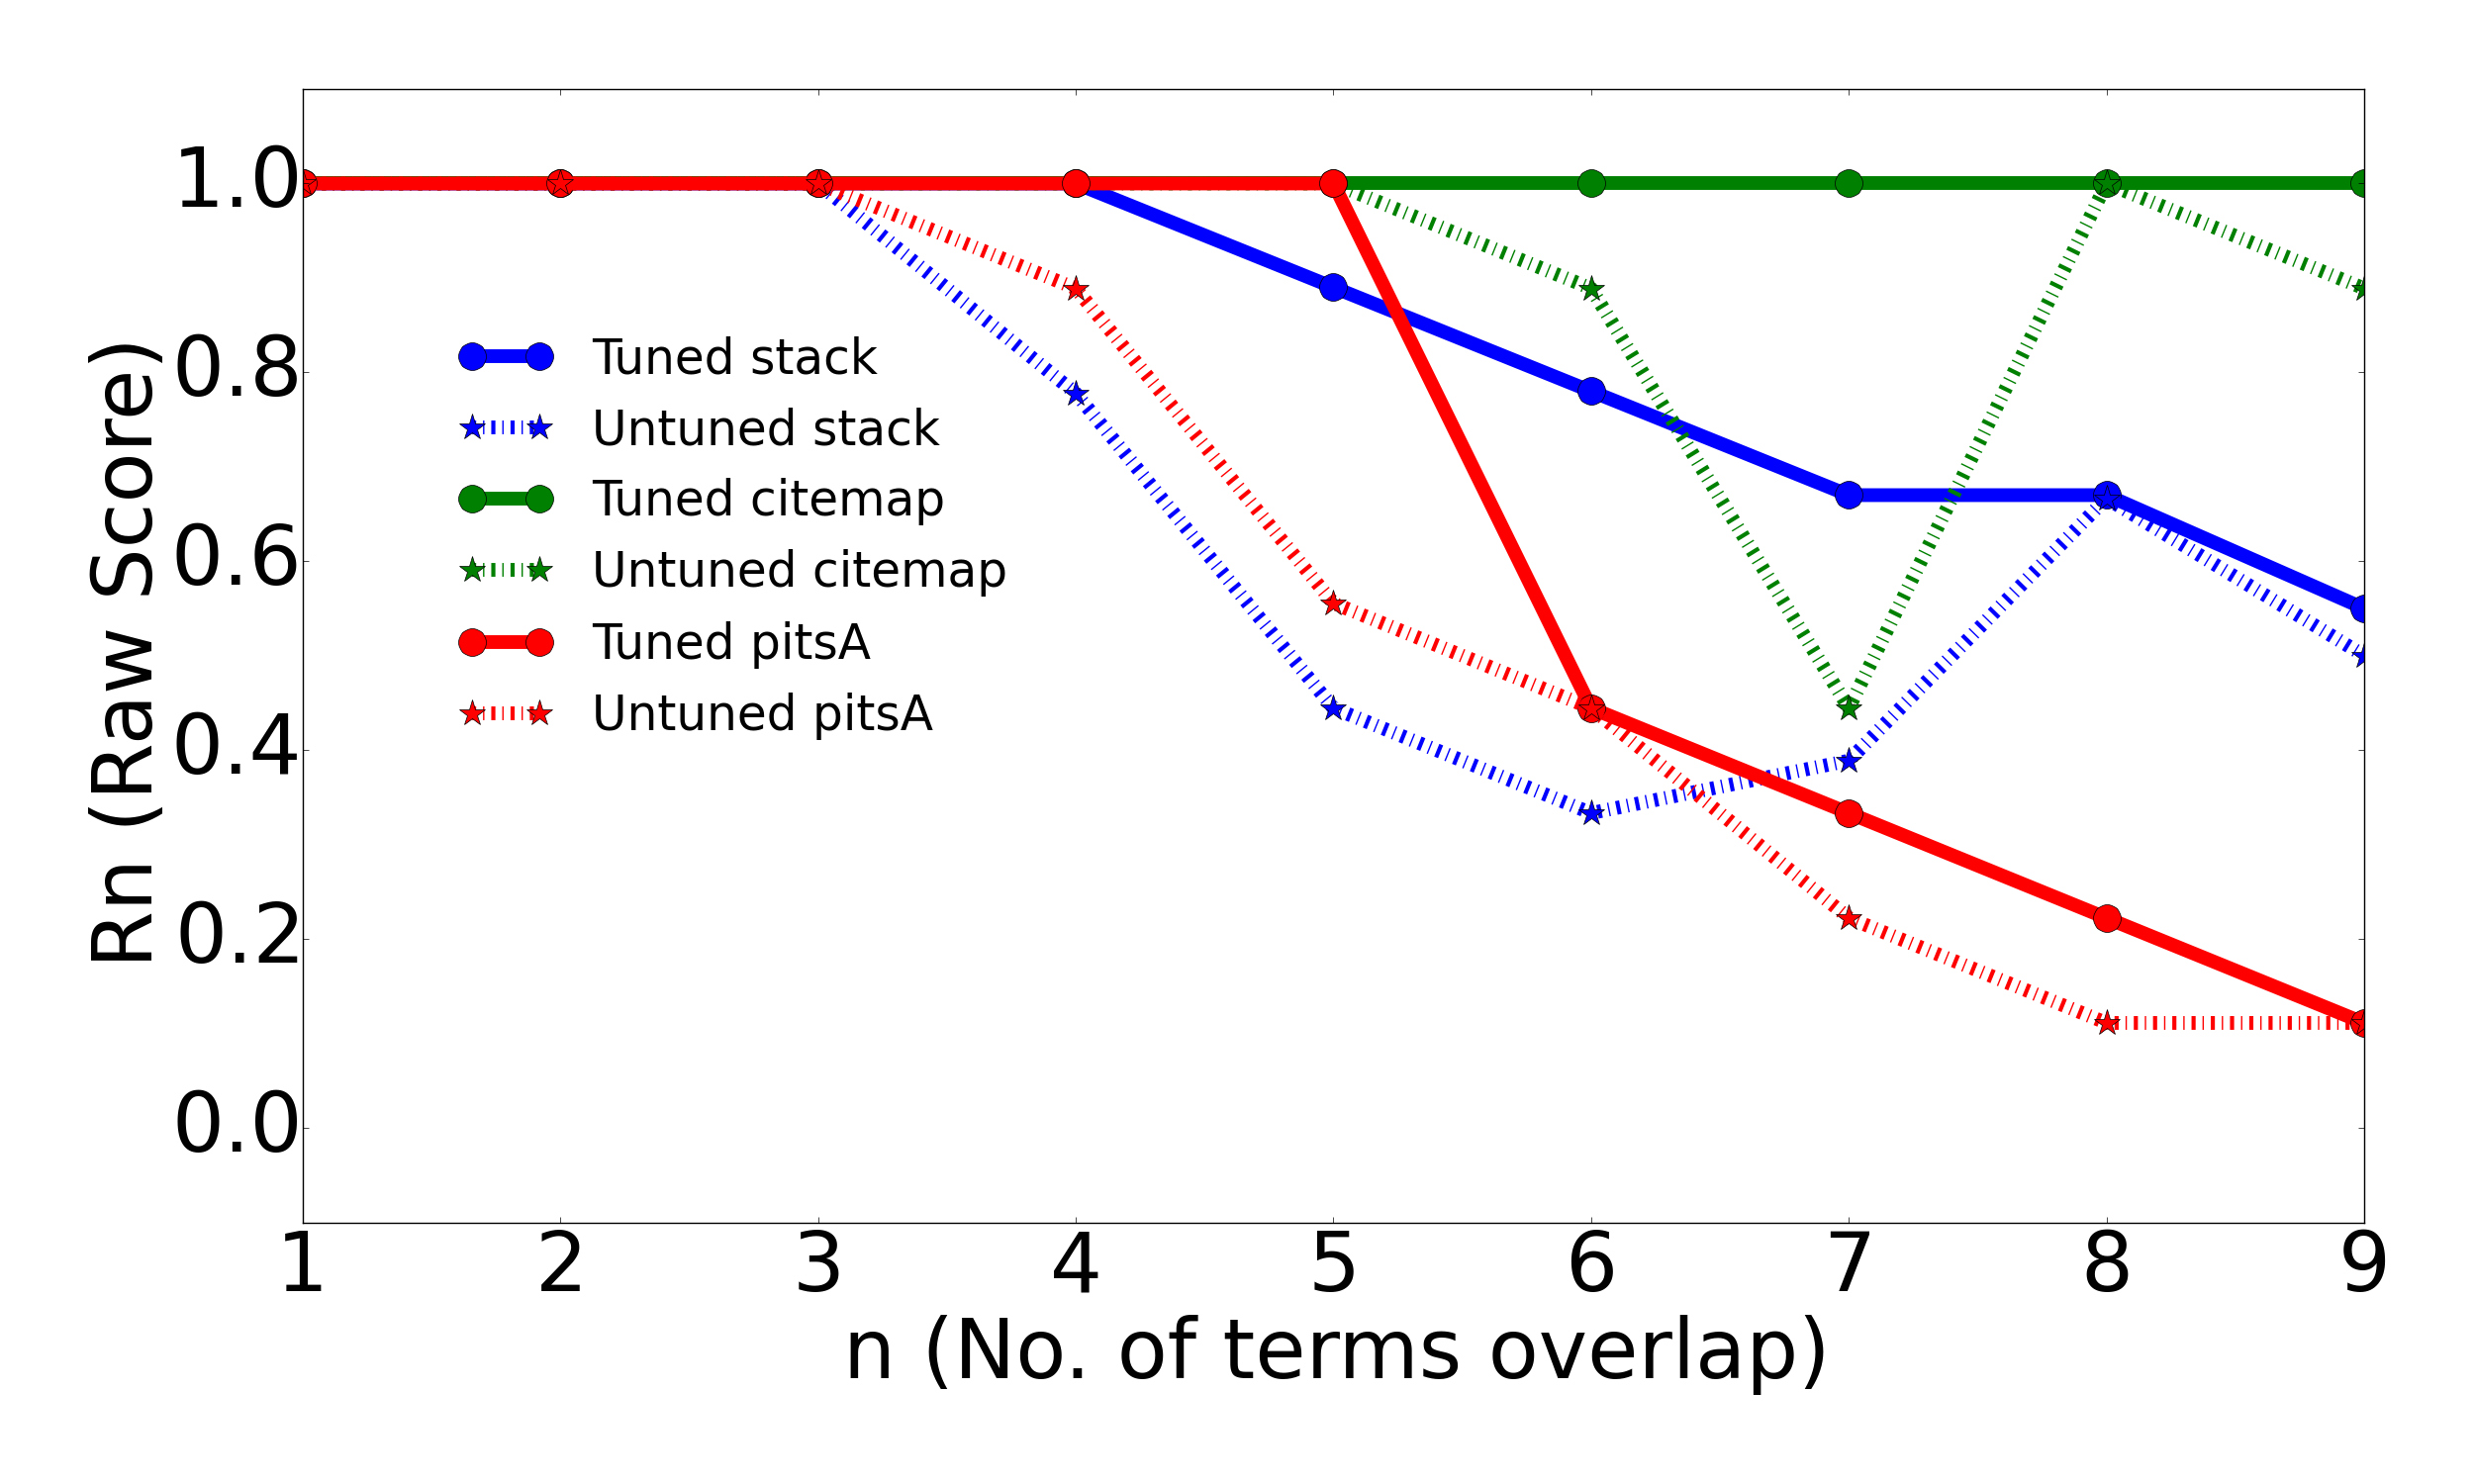
\includegraphics[width=\linewidth]{./fig/spark.png}
  \caption{Spark Results}
  \label{python_spark}
\end{figure}

Figure \ref{python_spark} shows tuning results for Stackoverflow, Citemap, and PitsA 
   using Scala/Spark cluster (for results on other data sets, see https://goo.gl/UVaql1).
   
  Another useful comparison is to change the internal of the LDA, sometimes using VEM sampling and other times using Gibbs sampling.


\begin{figure}[!htbp]
  \captionsetup{justification=centering}
  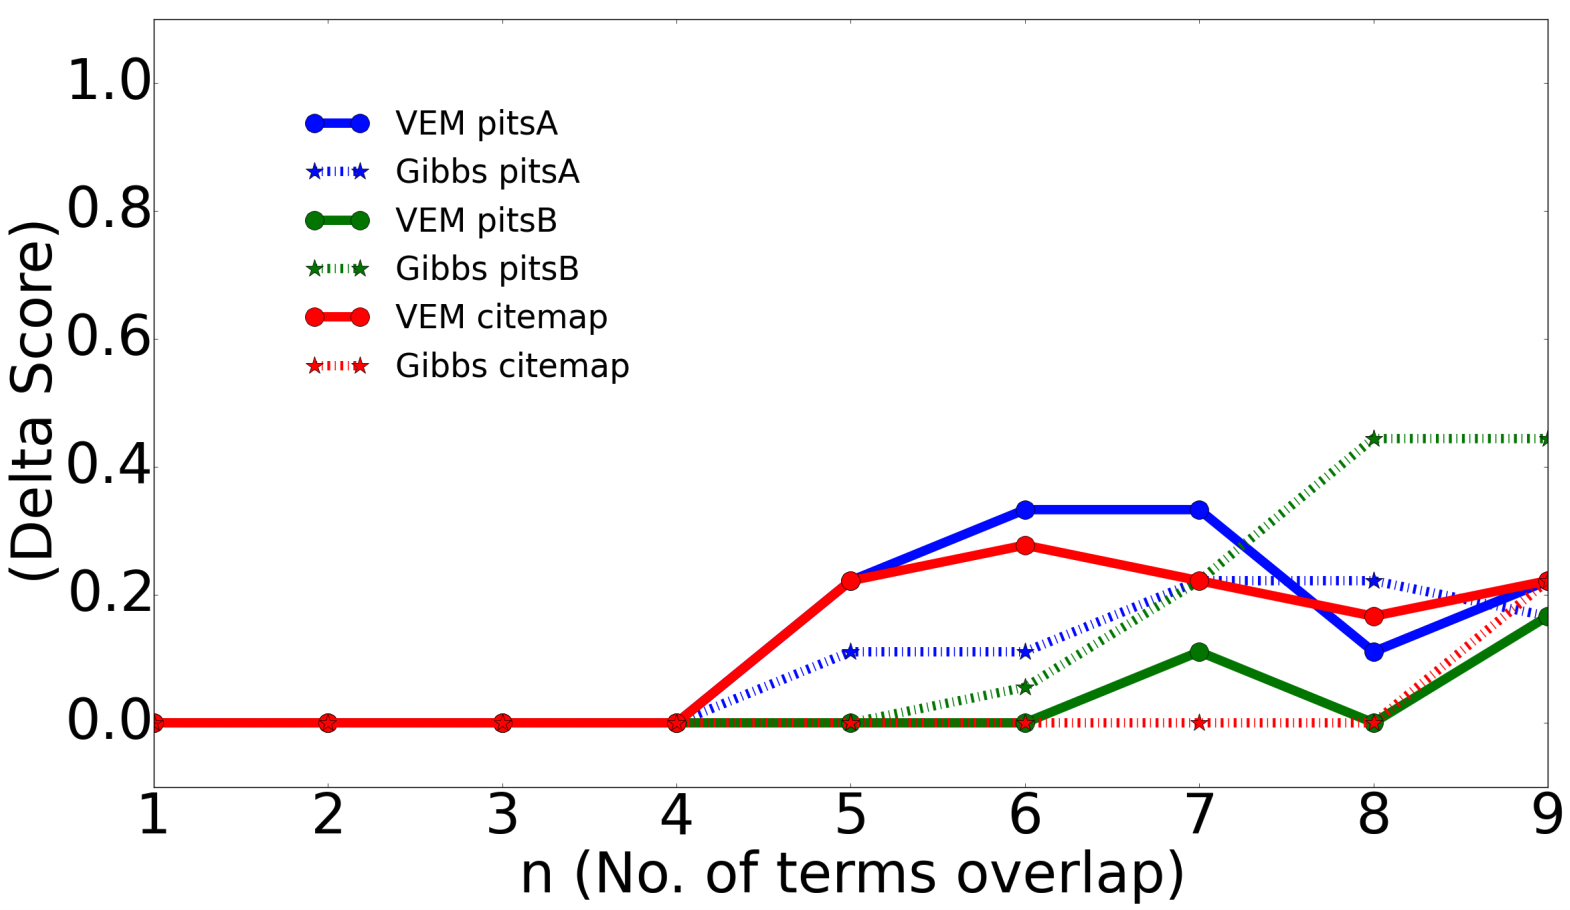
\includegraphics[width=\linewidth]{./fig/gibbs_vem1.png}
  \caption{GIBBS vs VEM}
  \label{gibbs_vem}
\end{figure}


  Figure~\ref{gibbs_vem} compares the  VEM vs Gibbs sampling (for results on other datasets, see https://goo.gl/faYAcg).
   
   When compared with the Python/desktop results of
   Figure~\ref{fig:delta} we see the same patterns:
   \bi
 \item Tuning never makes stability worse.
 \item Sometimes, it dramatically improves it (in particular, see the Citemap results
   of  Figure~\ref{python_spark}).
   \ei
   That said, there are some deltas between VEM and Gibbs where it seems tuning
   is more important for VEM than Gibbs (evidence: the improvements seen after
   tuning are largest for the  VEM results of  Figure~\ref{gibbs_vem} and at  https://goo.gl/faYAcg).

\begin{lesson}
  Instability is not due to any quirk in the implementation of LDA. Instability is consistent and LDADE can stabilize. 
\end{lesson}

\begin{figure}[!b]
  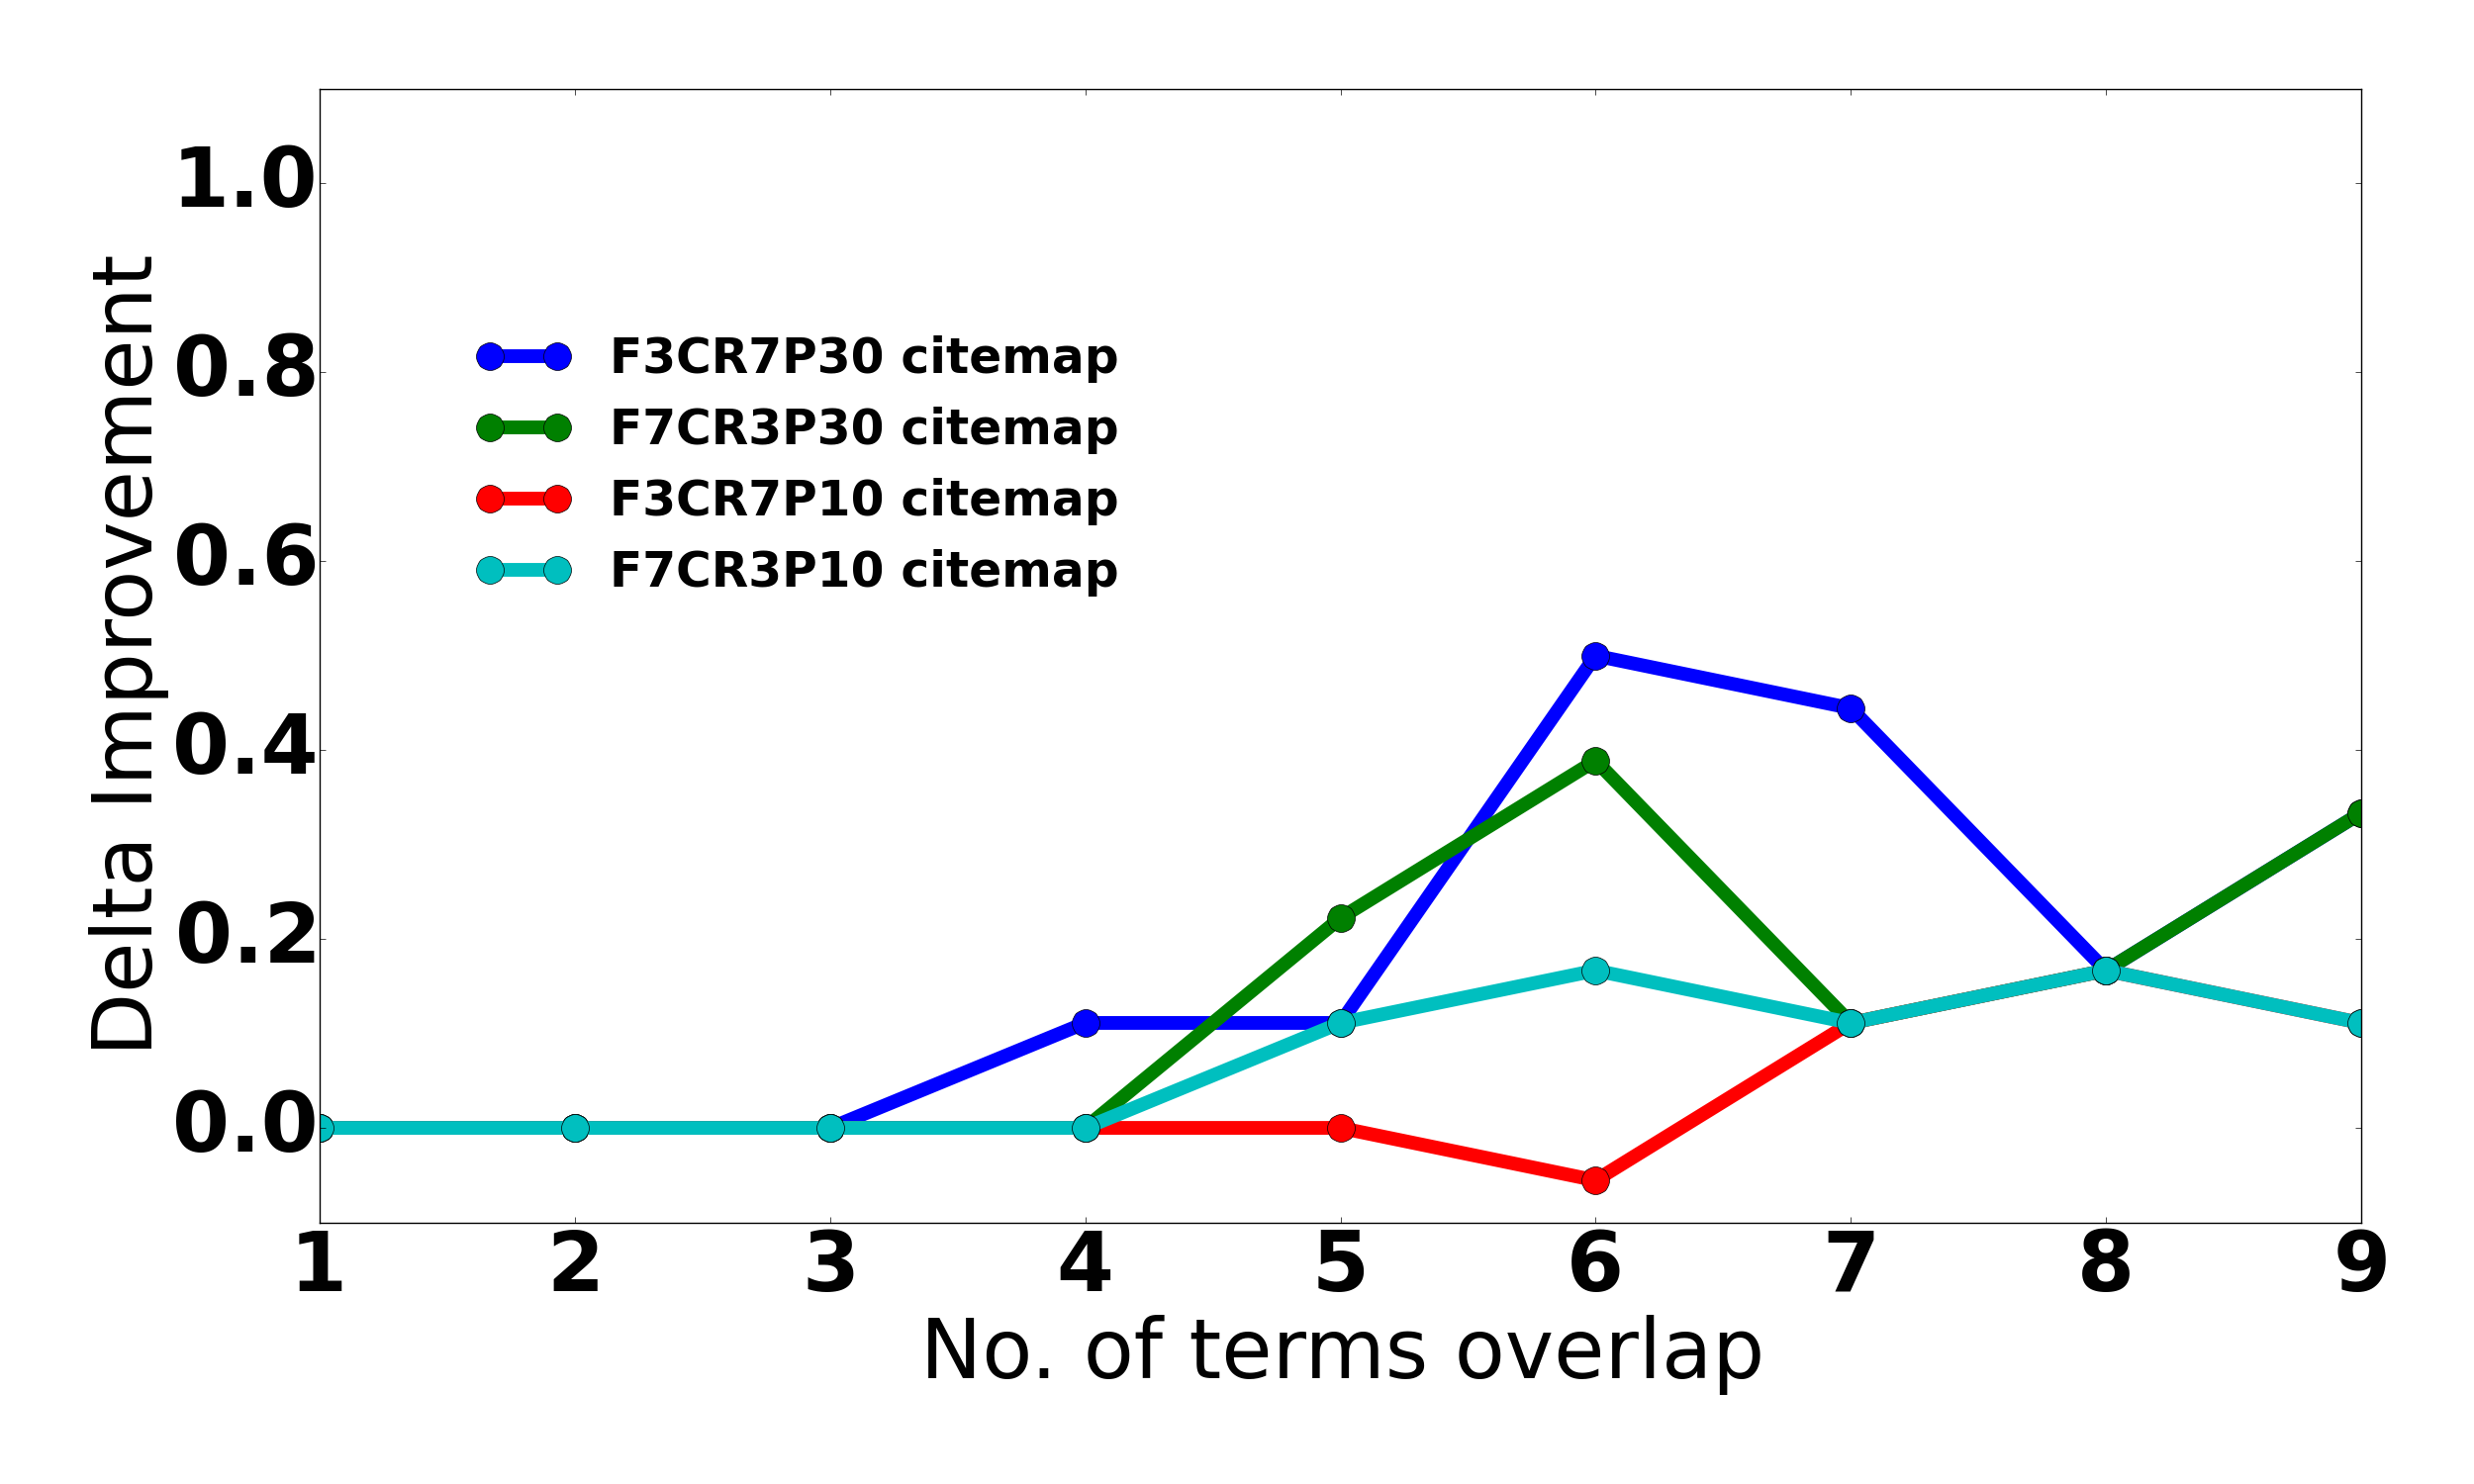
\includegraphics[width=\linewidth]{./fig/citemap.png}
  \caption{Terms vs Delta Improvement using Different settings of DE}
  \label{fig:RQ4}
\end{figure}

\begin{figure*}[!t]
    \centering
  \begin{minipage}{.49\textwidth}
        \captionsetup{labelsep=space,justification=centering}
        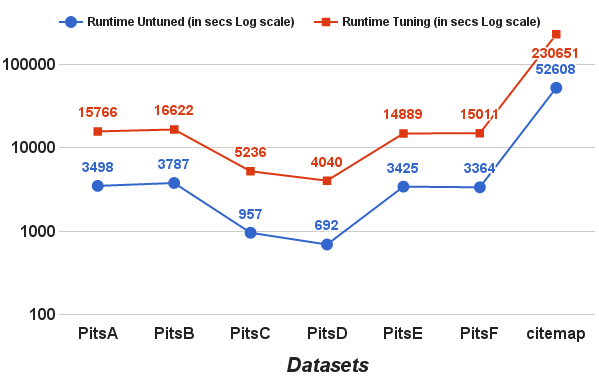
\includegraphics[width=\linewidth]{./fig/Run_VEM_sci.png}
  \caption{VEM: Datasets vs Runtimes}
  \label{RQ5 VEM}
  \end{minipage}
  \begin{minipage}{.49\textwidth}
        \captionsetup{justification=centering}
        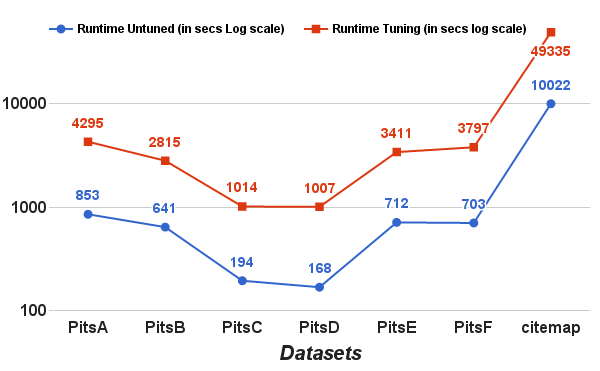
\includegraphics[width=\linewidth]{./fig/Run_gibbs_sci.png}
  \caption{Gibbs: Datasets vs Runtimes}
  \label{RQ5 Gibbs}
    \end{minipage}%
    
\end{figure*}

\subsection{\textbf{RQ6: Is  tuning  easy?}}


The DE literature
recommends using a population size $np$ that is ten times larger than the number of parameters being
optimized~\cite{storn1997differential}.  For example, when tuning $k,\alpha$ and $\beta$,
the DE literature is recommending $np=30$.
Figure~\ref{fig:RQ4} explores $np=30$ vs the $np=10$ we use in Algorithm 2
(as well as some other variants of DE's $F$ and $CR$ parameters).
The figure shows results just for Citemap and, for space reasons, results
relating to other data sets are shown at https://goo.gl/HQNASF.
After reviewing the results from all the datasets, we can say that there isn't much of an improvement by using different $F$, $CR$, and Population size. So our all other experiments used $F=0.7$, $CR=0.3$ and $np = 10$.
Also:

\begin{lesson}
  Finding stable parameters for
  topic models is easier than standard optimization tasks.
\end{lesson}

\subsection{\textbf{RQ7: Is tuning extremely slow?}}

Search-based SE methods can be very slow. Wang et al.~\cite{wang2013searching} once needed 15
years of CPU time to find and verify the tunings required for software
clone detectors. Sayyad et al.~\cite{sayyad2013scalable} routinely used
$10^6$ evaluations (or more) of their models in order to extract
products from highly constrained product
lines. Hence, before recommending any
search-based method, it is wise to consider the runtime cost of that
recommendation.

To understand our timing results, recall that untuned and tuned LDA use
Algorithm~1 and Algorithm~2 respectively. Based on the psuedocode
shown above, our pre-experimental expectation is that
tuning will be three times slower than not tuning.
 
Figures \ref{RQ5 VEM} and \ref{RQ5 Gibbs} check if that theoretical
holds true in practice. Shown in blue and red are the
  runtimes required to run LDA untuned and tuned (respectively).  The
  longer runtimes (in red) include the times required for DE to find
  the tunings. Overall, tuning slows down LDA by a factor of up to
  five (which is very close to our theoretical prediction).
  Hence, we say:

  
  \begin{lesson}
    Theoretically and empirically, tuning LDA costs three to five times more runtime
    as much as using untuned LDA.
  \end{lesson}

  While this is definitely more than not using DE, but this may not be an arduous increase
  given modern cloud computing environments.
  

\subsection{\textbf{RQ8: Should topic modeling be used ``off-the-shelf'' with their default tunings?}}

  Figure~\ref{fig:delta} shows that there is much benefit in tuning.
  Figures \ref{RQ3:k}, \ref{RQ3:a}, and \ref{RQ3:b} show that
  the range of ``best'' tunings is very dataset-specific. Hence, for a new dataset,
  the off-the-shelf tunings
  may often fall far from the useful range.
  Figures \ref{RQ5 VEM} and \ref{RQ5 Gibbs} show that tuning is definitely
  slower than otherwise, but the overall cost is not prohibitive.
  Hence:
  \begin{lesson}
    Whatever the goal is, whether using the learned topics, or cluster distribution for classification
    we cannot recommend using ``off-the-shelf'' LDA.
  \end{lesson}


\section{Threats to Validity}
\label{sect:validity}

As with any empirical study, biases can affect the final
results. Therefore, any conclusions made from this work must be considered with the following issues in mind:

\textbf{\textit{Sampling bias}} threatens any experiment; i.e., what matters there may not be true here. For example,
the data sets used here come after various pre-processing steps and could change if pre-processed differently. And that is why, all our datasets can be downloaded from the footnotes of this paper and researchers can explore further. Even though we used so many data sets, there could be other datasets for which our results could be wrong or have lesser improvement.

\textbf{\textit{Learner bias}}: For running LDA, we selected other parameters as default which are of not much importance. But there could be some datasets where by tuning them there could be much larger improvement. And for RQ2, we only experimented with linear kernel SVM. There could be other classifiers which can change our conclusions. Data Mining is a large and active field and any single study can only use a small subset of the known data miners.

\textbf{\textit{Evaluation bias}}: This paper uses topic similarity ($\Re_n$) and F2 measures of evaluation but there are other measures which are used in software engineering which
includes perplexity, performance, accuracy, etc. Assessing
the performance of stable LDA is a clear direction for future work.

\textbf{\textit{Order bias}}: With each dataset, how data samples are picked and put into LDA is completely random. Since this paper also consider input order effects, though there could be times when the input order could be with lesser variance. To mitigate this order bias, we ran the experiment 10 times by randomly changing the order of the data samples each time.


Another threat to validity of this work is that it is a quirk of the control
parameters used within our DE optimizer.
We have some evidence that this is not the case.
Figure~\ref{fig:RQ4} and https://goo.gl/HQNASF explored a range of DE tunings and found
little difference across that range. Also, Table~V explores another choice within DE -- how
many evaluations to execute before terminating DEs. All the results in this paper use an
evaluation budget of 30 evaluations. Table~V
compares results across different numbers of evaluations. While clearly,
the more evaluations the better, there is little improvement after the
30 evaluations used in this paper.

\begin{table}[!htbp]
\scriptsize
\begin{center}
\begin{tabular}{|c|c|c|c|c|}
\hline 
\textbf{Datasets\textbackslash Evaluations} & \textbf{10} & \textbf{20} & \textbf{30} &
\textbf{50} \\[0.5ex]
\hline
PitsA & 0.9 & 0.9 & 1.0 & 1.0\\ 
\hline
PitsB & 0.9 & 0.9 & 0.9 & 1.0 \\
\hline
PitsC & 0.9 & 1.0 & 1.0 & 1.0\\ 
\hline
PitsD & 0.9 & 1.0 & 1.0 & 1.0\\ 
\hline
PitsE & 0.9 & 0.9 & 1.0 & 1.0\\
\hline
PitsF & 0.9 & 0.9 & 0.9 & 0.9\\
\hline
Citemap & 0.67 & 0.67 & 0.77 & 0.77\\
\hline
Stackoverflow & 0.6 & 0.7 & 0.8 & 0.8\\
\hline
\end{tabular}
\end{center}
\caption{Evaluations vs Stability Scores}
\label{tb:tablename1}
\end{table}

The conclusions of this paper are based on a finite number of data sets and it is possible
that other data might invalidate our conclusions. As with all analytics papers, any researcher can do is to make their conclusions and materials public, then encourage
other researchers to repeat/refute/improve their conclusions.

\section{Conclusion and Future Work}

Based on the above, we offer a specific and general conclusion. Most specifically, we recommend 
\bi

\item  
Any study that shows the topics learned from LDA, and uses them to make a particular
conclusion, needs to first tune LDA. We say this since the topics learned from untuned LDA are unstable, i.e. different input orderings will lead to different conclusions. However, after tuning, stability can be greatly increased.
\item Unlike the advise of Lukins et al.~\cite{lukins2010bug}, LDA topics should not be reported as the top ten words.
  Due to order effects, such a report can be highly incorrect.
  Our results show that up to eight words can be reliably reported, but only
  after tuning for stability using tools like LDADE.
 \item Any other studies which are making use of these topic distribution for classification results need to be tuned first before using them in their further tasks.
\item Do not download someone else's pre-tuned LDA since, as shown here,  the best LDA tunings vary from data set to data set.
\item These results demand us to visit the previous case studies which have used LDA using ``off-the-shelf'' parameters to rerun by tuning these parameters using automated tools like LDADE.
    
\ei
Our experience is that this recommendation is not an arduous demand since tuning adds less than a factor of five to the total run times of an LDA study.

More generally, we comment that the field of software analytics needs to make far more use of search-based software engineering in order
to tune their learners. In other work, Fu et al. have shown that tuning significantly helps defect prediction~\cite{fu2016tuning} and an improvement also shown for LDA~\cite{panichella2013effectively}. In this work, we have shown that tuning significantly helps topic modeling by mitigating a systematic error in LDA  (order effects that lead to unstable topics). The implication of this study for other software analytics tasks is now an open
and pressing issue. 
In how many domains can search-based SE dramatically improve software analytics?


\section*{Acknowledgements}
		The work is partially funded by NSF award \#1506586.
	

\bibliographystyle{elsarticle-num}
\medskip
\bibliography{main}

\end{document}
